%% bare_conf.tex
%% V1.3
%% 2007/01/11
%% by Michael Shell
%% See:
%% http://www.michaelshell.org/
%% for current contact information.
%
%
%% This is a skeleton file demonstrating the use of IEEEtran.cls
%% (requires IEEEtran.cls version 1.7 or later) with an IEEE conference paper.
%%
%% Support sites:
%% http://www.michaelshell.org/tex/ieeetran/
%% http://www.ctan.org/tex-archive/macros/latex/contrib/IEEEtran/
%% and
%% http://www.ieee.org/

%%*************************************************************************
%% Legal Notice:
%% This code is offered as-is without any warranty either expressed or
%% implied; without even the implied warranty of MERCHANTABILITY or
%% FITNESS FOR A PARTICULAR PURPOSE! 
%% User assumes all risk.
%% In no event shall IEEE or any contributor to this code be liable for
%% any damages or losses, including, but not limited to, incidental,
%% consequential, or any other damages, resulting from the use or misuse
%% of any information contained here.
%%
%% All comments are the opinions of their respective authors and are not
%% necessarily endorsed by the IEEE.
%%
%% This work is distributed under the LaTeX Project Public License (LPPL)
%% ( http://www.latex-project.org/ ) version 1.3, and may be freely used,
%% distributed and modified. A copy of the LPPL, version 1.3, is included
%% in the base LaTeX documentation of all distributions of LaTeX released
%% 2003/12/01 or later.
%% Retain all contribution notices and credits.
%% ** Modified files should be clearly indicated as such, including  **
%% ** renaming them and changing author support contact information. **
%%
%% File list of work: IEEEtran.cls, IEEEtran_HOWTO.pdf, bare_adv.tex,
%%                    bare_conf.tex, bare_jrnl.tex, bare_jrnl_compsoc.tex
%%*************************************************************************

% *** Authors should verify (and, if needed, correct) their LaTeX system  ***
% *** with the testflow diagnostic prior to trusting their LaTeX platform ***
% *** with production work. IEEE's font choices can trigger bugs that do  ***
% *** not appear when using other class files.                            ***
% The testflow support page is at:
% http://www.michaelshell.org/tex/testflow/



% Note that the a4paper option is mainly intended so that authors in
% countries using A4 can easily print to A4 and see how their papers will
% look in print - the typesetting of the document will not typically be
% affected with changes in paper size (but the bottom and side margins will).
% Use the testflow package mentioned above to verify correct handling of
% both paper sizes by the user's LaTeX system.
%
% Also note that the "draftcls" or "draftclsnofoot", not "draft", option
% should be used if it is desired that the figures are to be displayed in
% draft mode.
%
\documentclass[10pt, conference, compsocconf]{IEEEtran}
% Add the compsocconf option for Computer Society conferences.
%
% If IEEEtran.cls has not been installed into the LaTeX system files,
% manually specify the path to it like:
% \documentclass[conference]{../sty/IEEEtran}


\usepackage[tight,footnotesize]{subfigure}
\usepackage{calc}
\usepackage{amstext}
\usepackage[cmex10]{amsmath}
%\usepackage{amsthm}
%\usepackage{multicol}
\usepackage{pslatex}
\usepackage{color}
\usepackage{graphicx}
%\usepackage[small]{caption}
\usepackage{booktabs}
%\usepackage{algorithm}
%\usepackage[noend]{algpseudocode}
\usepackage[linesnumbered]{algorithm2e}
\usepackage{epstopdf}
\usepackage{float}
\usepackage{flushend}

\newtheorem{theorem}{Theorem}
\newtheorem{corollary}{Corollary}[theorem]


\newcommand{\zh}{\textcolor{red}}

% Some very useful LaTeX packages include:
% (uncomment the ones you want to load)


% *** MISC UTILITY PACKAGES ***
%
%\usepackage{ifpdf}
% Heiko Oberdiek's ifpdf.sty is very useful if you need conditional
% compilation based on whether the output is pdf or dvi.
% usage:
% \ifpdf
%   % pdf code
% \else
%   % dvi code
% \fi
% The latest version of ifpdf.sty can be obtained from:
% http://www.ctan.org/tex-archive/macros/latex/contrib/oberdiek/
% Also, note that IEEEtran.cls V1.7 and later provides a builtin
% \ifCLASSINFOpdf conditional that works the same way.
% When switching from latex to pdflatex and vice-versa, the compiler may
% have to be run twice to clear warning/error messages.






% *** CITATION PACKAGES ***
%
%\usepackage{cite}
% cite.sty was written by Donald Arseneau
% V1.6 and later of IEEEtran pre-defines the format of the cite.sty package
% \cite{} output to follow that of IEEE. Loading the cite package will
% result in citation numbers being automatically sorted and properly
% "compressed/ranged". e.g., [1], [9], [2], [7], [5], [6] without using
% cite.sty will become [1], [2], [5]--[7], [9] using cite.sty. cite.sty's
% \cite will automatically add leading space, if needed. Use cite.sty's
% noadjust option (cite.sty V3.8 and later) if you want to turn this off.
% cite.sty is already installed on most LaTeX systems. Be sure and use
% version 4.0 (2003-05-27) and later if using hyperref.sty. cite.sty does
% not currently provide for hyperlinked citations.
% The latest version can be obtained at:
% http://www.ctan.org/tex-archive/macros/latex/contrib/cite/
% The documentation is contained in the cite.sty file itself.






% *** GRAPHICS RELATED PACKAGES ***
%
\ifCLASSINFOpdf
  % \usepackage[pdftex]{graphicx}
  % declare the path(s) where your graphic files are
  % \graphicspath{{../pdf/}{../jpeg/}}
  % and their extensions so you won't have to specify these with
  % every instance of \includegraphics
  % \DeclareGraphicsExtensions{.pdf,.jpeg,.png}
\else
  % or other class option (dvipsone, dvipdf, if not using dvips). graphicx
  % will default to the driver specified in the system graphics.cfg if no
  % driver is specified.
  % \usepackage[dvips]{graphicx}
  % declare the path(s) where your graphic files are
  % \graphicspath{{../eps/}}
  % and their extensions so you won't have to specify these with
  % every instance of \includegraphics
  % \DeclareGraphicsExtensions{.eps}
\fi









% correct bad hyphenation here
\hyphenation{op-tical net-works semi-conduc-tor}


\begin{document}
%
% paper title
% can use linebreaks \\ within to get better formatting as desired

\title{\uppercase{A systematic Fault-tolerant Computational Model For Both Crash Failures and Silent Data Corruption}}

% author names and affiliations
% use a multiple column layout for up to two different
% affiliations

\author{\IEEEauthorblockN{Xiaolong Cui, Zaeem Hussain, Taieb Znati, Rami Melhem}
\IEEEauthorblockA{Computer Science Department\\
University of Pittsburgh\\
Pittsburgh, USA\\
Email: \{mclarencui, zaeemhussain, znati, melhem\}@cs.pitt.edu}
%\and
%\IEEEauthorblockN{Authors Name/s per 2nd Affiliation (Author)}
%\IEEEauthorblockA{line 1 (of Affiliation): dept. name of organization\\
%line 2: name of organization, acronyms acceptable\\
%line 3: City, Country\\
%line 4: Email: name@xyz.com}
}

% conference papers do not typically use \thanks and this command
% is locked out in conference mode. If really needed, such as for
% the acknowledgment of grants, issue a \IEEEoverridecommandlockouts
% after \documentclass

% for over three affiliations, or if they all won't fit within the width
% of the page, use this alternative format:
% 
%\author{\IEEEauthorblockN{Michael Shell\IEEEauthorrefmark{1},
%Homer Simpson\IEEEauthorrefmark{2},
%James Kirk\IEEEauthorrefmark{3}, 
%Montgomery Scott\IEEEauthorrefmark{3} and
%Eldon Tyrell\IEEEauthorrefmark{4}}
%\IEEEauthorblockA{\IEEEauthorrefmark{1}School of Electrical and Computer Engineering\\
%Georgia Institute of Technology,
%Atlanta, Georgia 30332--0250\\ Email: see http://www.michaelshell.org/contact.html}
%\IEEEauthorblockA{\IEEEauthorrefmark{2}Twentieth Century Fox, Springfield, USA\\
%Email: homer@thesimpsons.com}
%\IEEEauthorblockA{\IEEEauthorrefmark{3}Starfleet Academy, San Francisco, California 96678-2391\\
%Telephone: (800) 555--1212, Fax: (888) 555--1212}
%\IEEEauthorblockA{\IEEEauthorrefmark{4}Tyrell Inc., 123 Replicant Street, Los Angeles, California 90210--4321}}




% use for special paper notices
%\IEEEspecialpapernotice{(Invited Paper)}




% make the title area
\maketitle


\begin{abstract}
    With the concerted efforts from researchers in hardware, software, algorithm, and data management, HPC is moving towards extreme-scale, featuring a computing capability of quintillion ($10^{18}$) FLOPS. 
As we approach the new era of computing, however, several daunting scalability challenges remain to be conquered. Delivering extreme-scale performance will require a computing platform that supports billion-way parallelism, necessitating a dramatic increase in the number of computing, storage, and networking components. At such a large scale, failure would become a norm rather than an exception, driving the system to significantly lower efficiency with unprecedented amount of power consumption. %The frequency and diversity of failures,  as well as the challenge of power, call for rethinking of the fault tolerance problem. 

To tackle this challeng, we propose an adaptive and power-aware algorithm, referred to as Lazy Shadowing, as an efficient and scalable approach to achieve high-levels of resilience, through forward progress, in extreme-scale, failure-prone computing environments. 
Lazy Shadowing associates with each process a ``shadow" (process) that executes at a reduced rate, and opportunistically rolls forward each shadow to catch up with the its leading process during failure recovery.
%overlaps the recovery time after each failure with the time needed to roll forward the shadows to a consistent state.
Compared to existing fault tolerance methods, our approach can achieve 20\% energy saving with potential reduction in solution time at scale.

\end{abstract}


\begin{IEEEkeywords}
Fault tolerance; Shadow Computing; Silent data corruption; Extreme-scale; Power awareness
\end{IEEEkeywords}


% For peer review papers, you can put extra information on the cover
% page as needed:
% \ifCLASSOPTIONpeerreview
% \begin{center} \bfseries EDICS Category: 3-BBND \end{center}
% \fi
%
% For peerreview papers, this IEEEtran command inserts a page break and
% creates the second title. It will be ignored for other modes.
\IEEEpeerreviewmaketitle

\section{Introduction}
\label{sec:intro}
As our reliance on IT continues to increase, the complexity and urgency of the problems our society will face 
in the future drives us to build more powerful and accessible computer systems. Among the different types of 
computer systems, High Performance Computing (HPC) and Cloud Computing systems are the two most powerful ones. 
For both, the computing power attributes to the massive amount of parallelism, which is enabled by 
the massive amount of CPU cores, memory modules, communication devices, storage components, etc. 

Since CPU frequency flattened out in early 2000s, parallelism has become the ``golden rule" to boost performance. 
In HPC, Terascale performance was achieved in the late 90’s with fewer than 10,000 heavyweight single-core processors. 
A decade later, petascale performance required about ten times more processors with multiple cores on each processor. Nowadays, a race
is underway to build the world's first exascale machine to accelerate scientific discoveries and breakthroughs. It is 
projected that an exascale machine will achieve billion-way parallelism by using one million sockets each supporting 
1,000 cores~\cite{doe_ascr_exascale_2011,top_ten_2014}. 

Similar trend is happening in Cloud Computing. 
As the demand for Cloud Computing accelerates, cloud service providers  
will be faced with the need to expand their underlying infrastructure to ensure the expected levels of performance, reliability and cost-effectiveness. 
As a result, lots of large-scale data centers have been and are being built by IT companies
to exploit the power and economies of scale. 
For example, Google, Facebook, and Rackspace have hundreds of thousands 
of web servers in dedicated data centers to support their business. 

Unfortunately, several challenging issues come with the increase in system scale. As today's HPC and Cloud Computing systems grow to 
meet tomorrow's compute power demand, the behavior of the systems will be increasingly difficult to specify, predict and manage. 
This upward trend, in terms of scale and complexity, has a direct negative effect on the overall system reliability. 
%Even with the expected improvement in the reliability of future computing technology, the rate of system level failures will 
%dramatically increase with the number of components, possibly by several orders of magnitude. 
At the same time, the rapid 
growing power consumption, as a result of the increase in system components, is another major concern. 
%It is reported that 
%the power required to run the machines as well as cool them has become the largest cost factor in a large-scale system's operating 
%expenses.  
At future extreme-scale, failure would become a norm rather than an exception, 
driving the system to significantly lower efficiency with unprecedented amount of power consumption. 

\section{Problem Statement}

The system scale needed to address our future computing needs will come at the cost of increasing complexity, unpredictability, 
and operating expenses. As we approach future extreme-scale computing, two of the biggest challenges will be system resilience and power 
consumption, both being direct consequences of the dramatic increase in the number of system components~\cite{exa_challenge_2010,snir2014addressing}. 

Regardless of the reliability of individual component, the system level failure rate will continue to increase as the number of 
components increases, possibly by several orders of magnitude. It is projected that the Mean Time Between Failures (MTBF) of future extreme-scale systems will be at the order of hours or even minutes, meaning 
that many failures will occur every day~\cite{Bergman08exascalecomputing}. Without an efficient fault tolerance mechanism, faults will be so frequent that the applications running on the 
systems will be continuously interrupted, requiring the execution to be restarted every time there is a failure. 

Also thanks to the continuous growth in system components, there has been a steady rise in power consumption in large-scale distributed systems. 
In 2005, the peak power consumption of a single supercomputer reached 3.2 Megawatts. This number was doubled only after 5 years, and reached 17.8 
Megawatts with a machine of 3,120,000 cores in 2013. Recognizing this rapid upward trend, the U.S. Department of Energy has set 20 
megawatts as the power limit for future exascale systems, 
challenging the research community to provide a 1000x improvement in performance with only a 10x increase in power~\cite{exa_challenge_2010}. 
This huge imbalance makes system power a leading design constraint on the path to exascale. 

Today, two approaches exist for fault tolerance. The first approach is rollback recovery, which rolls back and restarts the execution 
every time there is a failure. This approach is often equipped with checkpointing to periodically save the execution state to a 
stable storage so that execution can be restarted from a recent checkpoint in the case of a failure~\cite{Elnozahy:02:Survey,kalaiselvi_sadhana_2000,Chandy:1985:DSD:214451.214456}. 
Although checkpointing is the most widely used technique in today's HPC systems, it may not scale to 
future extreme-scale systems~\cite{ferreira_sc_2011,elnozahy_dsc_2004,4367962}. Given the anticipated increase in system level failure rates and the time to checkpoint large-scale 
compute-intensive and data-intensive applications, the time required to periodically checkpoint an application 
and restart its execution will approach the system's MTBF~\cite{Cappello:2009:TER:1640402.1640428}. Consequently, applications will make little forward progress, thereby 
reducing considerably the overall system efficiency. 

The second approach, referred to as process replication, exploits hardware redundancy and executes multiple instances of the same task 
in parallel to overcome failure and guarantee that at least one task instance reaches completion~\cite{bartlett_1981_nonstop,tsai_isads_2011,ferreira_sc_2011}. Although this approach is extensively used 
to deal with failures in 
Cloud Computing and mission critical systems, it has 
never been used in any HPC system due to its low system efficiency. To replicate each process, process replication requires 
at least double the amount of compute nodes, which also increases the power consumption proportionally. 

Based on above analysis, neither of the two approaches is efficient for future extreme-scale systems. And unfortunately, neither 
of them addresses the power cap issue. 
Achieving high resilience to failures under strict power constraints is a daunting and critical challenge that requires new 
computational models with scalability, adaptability, and power-awareness in mind. 
 
\section{Research Overview}

There is a delicate interplay between fault tolerance and power consumption. Checkpointing and process replication require 
additional power to achieve fault tolerance. Conversely, it has been shown that lowering supply voltages, a commonly used 
technique to conserve power, increases the probability of transient faults~\cite{chandra2008defect,zhao2008reliability}. The trade-off between fault free operation and 
optimal power consumption has been explored in the literature~\cite{meneses2014energy,mills2014energy}. Limited insights have emerged, however, with respect to how 
adherence to application's desired QoS requirements affects and is affected by the fault tolerance and power consumption 
dichotomy. In addition, abrupt and unpredictable changes in system behavior may lead to unexpected fluctuations in performance, 
which can be detrimental to applications’ QoS requirements. The inherent instability of extreme-scale computing systems, 
in terms of the envisioned high-rate and diversity of faults, together with the demanding power constraints under which 
these systems will be designed to operate, calls for a 
reconsideration of the fault tolerance problem.

To this end, Mills, Znati, and Melhem have proposed a novel computational model, referred to as Shadow Replication, as a  
power-aware approach to achieve high-levels of resilience through forward progress~\cite{mills_2014_icnc,mills_2014_pdp,mills2014power}. Based on Dynamic Voltage and Frequency Scaling (DVFS)~\cite{Orgerie:2014:STI:2597757.2532637,4658633,LeSueur:2010:DVF:1924920.1924921}, Mills studied the computational model and its performance in terms of completion time and energy consumption in HPC systems. Through the use of analytical models, simulations, and experimentation, Mills demonstrated that Shadow Replication can achieve resilience more efficiently than both checkpointing and traditional replication when power is limited. However, in Mills' work Shadow Replication is limited to the use of DVFS, which has been shown to have multiple issues that question its viability~\cite{Eyerman:2011:FDU:1952998.1952999,Keller:EECS-2015-257,chandra2008defect,zhao2008reliability}. In addition, Mills' study is limited to HPC systems and focuses exclusively on minimizing energy consumption with constraints on time to completion. In contrast, QoS requirements for various computing systems can be expressed in multiple dimensions that go beyond time and energy. At the same time, an implementation is needed to verify the computational model both with and without failures. 


%In this thesis, our research objective is to simultaneously address the power and resilience challenges for future extreme-scale 
%systems so that both system efficiency and application QoS are guaranteed.
%To this end, we propose an adaptive and power-aware computational model, referred to as Lazy Shadowing, as an efficient and 
%scalable alternative to achieve high-levels of resilience, through forward progress, in extreme-scale, failure-prone 
%computing environments. 
%The basic tenet of Lazy Shadowing is to associate with each main process a suite of “shadows” whose size depends on the 
%``criticality" of the application and its performance requirements. Each shadow process is an exact replica of the original 
%main process. To tolerate failures, the main process and its associated shadow processes will execute in parallel, but on 
%different compute nodes. 
%The shadows initially execute at a reduced rate %via Dynamic Voltage Frequency and Scaling (DVFS) 
%to save power. 
%If the main process completes the task successfully, we will 
%terminate the shadows immediately. If the main process fails, however, we will promote one of the shadow processes to be a 
%new main process and possibly increase its execution rate to mitigate delay.

To address the above limitations, this thesis builds on the computational model of Shadow Replication, and seeks to simultaneously address the power and resilience challenges for future extreme-scale systems while guaranteeing system efficiency and application QoS.
Specifically, this thesis tries to answer 4 questions: 1) is Shadow Replication general enough to achieve objectives beyond time to completion; %, such as multiple simultaneous requirements defined in a SLA in the Cloud; 
2) how to enable Shadow Replication when DVFS is not viable, and ensure forward progress in failure-prone, extreme-scale systems; 3) is the computational model realistic in real environments; and 4) how to make the computational model reflective of the propensity of the processing elements to failures and adaptive to different environments and requirements.
With these questions in mind, 
I have studied different techniques to embody and augment the model, and developed analytical frameworks for different objectives in the Cloud and HPC environments~\cite{cui_2014_closer,cui_en7085151,cui_2016_scalcom}.
%Previously, we have formally defined the computational model, studied possible techniques to realize and optimize the idea, and 
%built analytical models for performance evaluation. 
To complete my thesis, I propose to extend the study in the following two aspects.
Firstly, I propose to implement a prototype in the context of Message Passing Interface (MPI), to validate the 
computational model as well as measure its performance in real environment. Secondly, I propose to study  
``smart shadowing" which adapts to the system configuration, application characteristics, and QoS requirement.
In summary, my thesis will consist of the following main components.

%\subsection{Lazy Shadowing: a novel fault-tolerant computational model (completed)}

%The basic tenet of Lazy Shadowing is to associate with each main process a suite of “shadows” whose size depends on the 
%``criticality" of the application and its performance requirements. Each shadow process is an exact replica of the original 
%main process. To tolerate failures, the main process and its associated shadow processes will execute in parallel, but on 
%different compute nodes. 
%The shadows initially execute at a reduced rate %via Dynamic Voltage Frequency and Scaling (DVFS) 
%to save power. 
%If the main process completes the task successfully, we will 
%terminate the shadows immediately. If the main process fails, however, we will promote one of the shadow processes to be a 
%new main process and possibly increase its execution rate to mitigate delay. This continues until the task completes. 

%Given that the failure rate of an individual node is much lower than the aggregate system failure, it is very likely that 
%the main process will always complete its execution successfully, thereby achieving fault tolerance at a significantly reduced 
%cost of power. Consequently, the high probability that shadows never have to complete the full task, coupled with the fact that 
%they initially only consume a minimal amount of power, dramatically increases a power-constrained system's tolerance to failure.

\subsection{Reward-based optimal Shadow Replication (completed)}
Shadow Replication is a flexible computational model that can achieve multi-dimensional QoS requirements. 
The major challenge resides in determining jointly the execution rates of all task instances, 
both before and after a failure occurs, with the objective to optimize performance, resilience, power consumption, or their combinations.
In this work we focus on the Service Level Agreement (SLA) requirements in the Cloud and develop a reward-based analytical framework, in order to derive the optimal execution rates for maximizing reward and minimizing energy 
costs under strict completion time constraints~\cite{cui_2014_closer,cui_en7085151}. 

%To define the reward-based analytical framework, we first define a failure model that considers the failure distribution of each process, and a power model that describes the power consumption characteristics under different states. Based on the failure model and power model, we then derive the expected income as a function of completion time, and the expected energy cost as a product of power and time. Lastly, the reward is defined as the optimization objective to balance between completion time and energy cost.  



\subsection{Lazy Shadowing (completed)}

Enabling Shadow Replication for resiliency in extreme-scale computing brings about a number of challenges and design decisions, including the applicability of this concept to a large number of tasks executing in parallel, 
the effective way to control shadows’ execution rates, and the runtime mechanisms and communications support to ensure efficient 
coordination between a main and its shadow. Taking into consideration the main characteristics of compute-intensive and 
highly-scalable applications, 
we devise novel ideas of shadow collocation and shadow leaping, and integrate them with Shadow Replication to form a more efficient and scalable paradigm that we call Lazy Shadowing~\cite{cui_2016_scalcom}.
%we design two novel techniques, referred to as shadow collocation and shadow leaping, 
%in order to achieve high tolerance to failures while minimizing delay and power consumption.

%To control the processes' execution rate, DVFS can be applied while each process resides on one core exclusively. 
%The effectiveness of DVFS, however, may be markedly 
%limited by the granularity of voltage control, the number of frequencies available, and the negative effects on 
%reliability. 
%An alternative is to collocate multiple processes on each core while keeping all the cores executing at maximum frequency. 
%Then time sharing can be used to achieve the desired execution rates for each collocated process. 
%Since this approach collocates multiple processes on a core, it simultaneously reduces the number of compute nodes and 
%the power consumption. 
%
%Furthermore, we identify a unique opportunity that ensures forward progress in failure-prone environments. Since each shadow process is associated with a main process, the lagging shadow can benefit from the faster execution 
%of the main with minimal overhead. Specifically, when a failure occurs, Lazy Shadowing takes advantage of 
%the recovery time and leaps forward each shadow by copying states from its associated main. This technique not only achieves forward 
%progress for the shadow processes at minimized power and delay, but also reduces the recovery time after each failure.

\subsection{lsMPI: an implementation in MPI (in progress)}

Though Lazy Shadowing has been evaluated analytically, a real implementation 
is necessary for validation and performance measurement in real systems. I am implementing a prototype of Lazy 
Shadowing as a runtime for Message Passing Interface (MPI). %, which is the de facto programming paradigm for HPC. 
%Instead of 
%a full-feature MPI implementation, the runtime is designed to be a separate layer between MPI and user application, in order 
%to take advantage of existing MPI performance optimizations that numerous researches have spent years on. 
The runtime will spawn 
the shadow processes at initialization phase, manage the coordination between main and shadow processes, 
and guarantee order and consistency for messages and non-deterministic events. With this implementation, we will perform thorough 
experiments to measure its runtime overhead as well as performance under failures.

\subsection{Smart shadowing (future)}
Lazy Shadowing is a flexible and adaptive computational model that deserves further investigation. Previous studies have shown that 
different nodes tend to have different failure probabilities, e.g., 19\% of the nodes account for 92\% of the machine check errors on Blue Waters~\cite{di2014lessons}. The reason 
is complicated and may attribute to the manufacture process, heterogeneous architecture, environment factors (e.g. temperature), 
and/or workloads. % I propose to apply machine learning techniques to learn the heterogeneity in failure distributions among a given 
%system's nodes. 
Under differernt failure distribution assumptions, I will study how the mapping from processes to physical cores can impact the performance and cost dichotomy. 
In addition, I will further consider allocating different number of shadow processes for different tasks to reduce cost while 
maintaining performance. 

\section{Contributions}
When completed, this thesis will make the following contributions:

\begin{itemize}
\item A reward-based framework for Shadow Replication to satisfy SLA requirements as well as maximize profit in Cloud Computing
\item Study of Lazy Shadowing as an enhanced model for future extreme-scale systems
\item A fully functional implementation of Lazy Shadowing for Message Passing Interface
\item Exploration of Lazy Shadowing's adaptivity to different environments, workloads, and QoS requirements. 
\end{itemize}


\section{OUTLINE}
\label{outline}
The rest of this proposal is organized as follow:  
Chapter \ref{chapter:background} reviews existing fault tolerance techniques in large-scale distributed systems, 
and Chapter \ref{chapter:shadowing} introduces the Shadow Replication computational model. In Chapter \ref{chapter:reward} we build a reward-based optimization framework for Shadow Replication in the Cloud environment.
In Chapter \ref{chapter:scale}, we introduce Lazy Shadowing which enhances Shadow Replication for extreme-scale systems. 
Implementation issues are discussed in Chapter \ref{chapter:implementation}. Adaptivity and smart shadowing are discussed in Chapter \ref{chapter:smart}.
%Chapter \ref{chapter:timeline} and \ref{chapter:summary} lists the timeline and concludes the proposal, respectively.
Chapter~\ref{chapter:summary}  concludes the proposal.










%\section{\uppercase{Related Work}}
%\label{sec:related_work}
%%Extreme-scale computing presents some unique challenges to fault tolerance as faults are no longer 
%an exceptional event \cite{ferreira_sc_2011}. 
Rollback and recovery is the predominate mechanism to achieve fault
tolerance in current HPC environments. In the most general form, rollback and recovery 
involves the periodic saving of the current system state, with the anticipation that
in the case of a failure, computation can be restarted from the most recently saved state \cite{Elnozahy:02:Survey}. %The identification of an error, before or during a checkpoint,
%requires that the application rollback to the previously completed checkpoint. 
Coordinated checkpointing is a popular approach for
its ease of implementation.
%Specifically, all processes
%coordinate with one another to produce individual states that satisfy the ``happens before"
%communication relationship \cite{chandy_trans_1972}, which is proved to provide a consistent global state.
%Essentially, the algorithm provides a method for all processes involved to stop operation ``at the same
%time" and transfer their system state to a stable storage. 
%The major benefit of coordinated
%checkpointing stems from its simplicity and ease of implementation. 
Its major drawback, however, is the
lack of scalability, as it requires global coordination
\cite{elnozahy_dsc_2004,riesen_sandia_2010}.
%hargrove2006berkeley}.


In uncoordinated checkpointing, processes record their states independently and postpone creating a 
globally consistent view until the recovery phase. The major advantage is the reduced overhead during fault free operation. However, the scheme requires that
each process maintains multiple checkpoints and message logs, necessary to construct a consistent 
state during recovery. It can also suffer the well-known domino effect 
 \cite{randell_domino_effect}. One hybrid approach, known as communication induced 
checkpointing, aims at reducing coordination overhead \cite{alvisi_ftc_1999}. The approach, however, may 
cause processes to store useless states. To address this 
shortcoming, ``forced checkpoints" have been proposed \cite{helary_rds_1997}. This approach, however,  may lead to unpredictable
checkpointing rates. Although well-explored, uncoordinated checkpointing has not been widely adopted
in HPC environments, due to its dependency on applications \cite{guermouche_2011_ipdps}.


One of the largest overheads in any checkpointing process is the time necessary to write the checkpointing 
to stable storage. Incremental checkpointing attempts
to address this by only writing the changes since previous checkpoint \cite{Agarwal:04:Adaptive,elnozahy_1992_manetho,li_trans_1994}. %This
%can be achieved using dirty-bit page flags \cite{plank_ftcs_1994,elnozahy_1992_manetho}. Hash based incremental checkpointing, on the other
%hand, makes use of hashes to detect changes \cite{nam_ftc_1997,Agarwal:04:Adaptive}. 
Another proposed scheme, known as in-memory checkpointing, minimizes the overhead of disk access~\cite{zheng_2004_ftccharm}.
%offloads the checkpointing process to a secondary task and only writes incremental checkpoints \cite{li_trans_1994}.
The main concern of these techniques is the increase in
memory requirement to support the simultaneous execution of the checkpointing and the application. It has been suggested that nodes in extreme-scale systems should be configured with fast local storage~\cite{doe_ascr_exascale_2011}. 
%, which
%improves the performance of checkpointing \cite{doe_ascr_exascale_2011}. 
Multi-level checkpointing, which consists of
writing checkpoints to multiple storage targets, can benefit from such a strategy \cite{Moody:10:SCR}. This,
however, may lead to increased failure rates of individual nodes and complicate the checkpoint writing process.
%Furthermore, it may complicate the checkpoint writing process and requires that the system track the
%current location of all process's checkpoints.


Our work is based on process replication, or state machine replication, which has long been used to provide fault tolerance in distributed and mission critical systems\cite{schneider_1990_tutorial}. %Replication can be used to detect and correct system failures that are otherwise undetectable,
%such as silent data corruption and Byzantine faults \cite{fiala_2012_sdc}. 
Recently, replication has been proposed as a
viable alternative to checkpointing in HPC \cite{ferreira_sc_2011,Cappello:09:Fault,fiala_2012_sdc}. 
In addition, full and partial
replication have also been used to augment existing checkpointing techniques, and to guard
against silent data corruption \cite{stearly_2012_partial,elliott_2012_cpr}.% There are several different implementations of
%replication in the widely used MPI library, each with their different tradeoffs and overheads. The
%overhead can be negligible or up to 70\% depending upon the communication patterns of the
%application \cite{engelmann2011redundant}. %Moreover, replication alone is not enough to guarantee fault tolerance since
%it is possible that all nodes executing a given process could fail simultaneously, thus
%replication is typically paired with some form of checkpointing. 
The most relevant works to ours is redundant multi-threading (RMT) whereby one leading thread of execution is running ahead of trailing threads \cite{reinhardt2000transient,Wadden:2014:RDE:2665671.2665686}. However, our approach is different in that it tunes the execution rates of the leading and trailing threads in a finer grain, in order to achieve a ``parameterized" trade-off between completion time and energy consumption. Further, we take advantage of the idle time during failure recovery and ``leap" the trailing threads to achieve forward progress%, largely improving performance in terms of both completion time and energy consumption. 
. This differs from RMT, of which the ``leaping" of the trailing thread results in extra overhead.
%To the best of our knowledge,
%Lazy Shadowing is the first attempt to explore a state-machine replication based framework
%that achieves a fine-grained tradeoff between time and hardware redundancy while meeting resilience and
%power requirements.


\section{Data-parallel programming paradigm}
\label{sec:execution_framework}
Data-intensive workloads represent a significant portion of today's large-scale computation. The applications range from business intelligence, bioinformatics, recommendation, to data streaming from large-scale simulations, distributed sensors, and social networks. To speed up scientific discoveries or to maximize commercial profits, many applications require that the data are processed in nearly real-time. 

Parallel computing frameworks, such as MapReduce, Dryad, and Spark, have been widely adopted for large-scale data analytics and batched stream processing~\cite{Dean2004,Isard2007,Zaharia180560,Bhatotia2011}. To efficiently handle the sheer amounts of data and simultaneously utilize a cluster of nodes and/or multiple cores within a node, these frameworks typically arrange a job into hundreds or thousands of tasks scheduled to execute in parallel, each processing one partition of the whole dataset\footnote{For iterative and graph algorithms, multiple stages of such parallel execution may be needed.}. This paradigm is depicted in Figure~\ref{fig:engine}.

\begin{figure}[!t]
  \begin{center}
      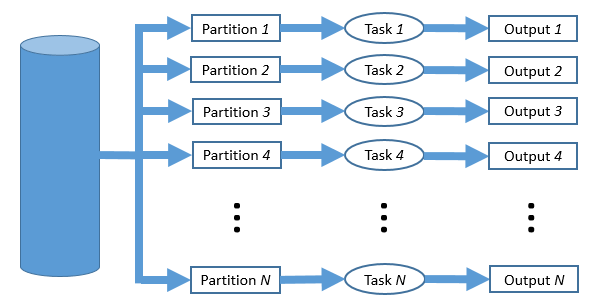
\includegraphics[width=0.8\columnwidth]{figures/engine}
  \end{center}
  \vskip -0.1in
  \caption{Parallel data processing paradigm.}
  \label{fig:engine}
  \vspace{-0.1in}
\end{figure}

The increasingly large scale of the Cloud data centers points to the growing interest in fault tolerance. Faults can be attributed to both hardware, such as manufacture defects and wear-down, and software, including bugs, race-condition, and deadlocks. Additionally, system overloading can also lead to unexpected behaviors, e.g., a low priority job may be terminated to accommodate a high priority job. Despite the cause, fault can be classified into two types based on its externally visible manifestation: 1) crash failure, which forces the target processor to stop immediately; 2) silent data corruption, which allows the target processor to continue execution but produce incorrect results.  

In today's parallel computing frameworks, re-execution on top of a heartbeat protocol is mainly used to provide fault tolerance and to deal with staggers. This approach works fine for system scales such that failures are rare and applications that are delay-tolerant. If failures are frequent, however, large delay can be incurred since one faulty task or stagger may delay the whole job execution. In addition, re-execution only handles crash failures. This is not acceptable for applications with strict response time requirements or vulnerable to silent data corruption. In contrast, Shadow Computing, if applied, will enable these frameworks to trade-off among multiple objectives, while respecting any hard or soft deadline and handling both types of failures. 

%For the development of analytical models and optimization frameworks in the following sections, we define necessary notations here. 



%\section{\uppercase{Dealing with crash failures}}
%\label{sec:crash}
%%\Section{Dealing with crash failures}

In data-intensive applications, input data are divided into multiple splits that can be processed in parallel. To deal with crash failures, the Soft Replication computational model can be applied, with one fast replica and one slow replica assigned to each data split. The fast and slow replicas for the same split will process the split from two opposite ends, and complete the processing by meeting in some middle point, if no failure occurs. If one process fails, however, its associated process can continue and process the remaining data, potentially with a higher execution rate to minimize delay.

\subsection{Notations}
Let $W$ denote the required workload to process one data split, which is often the unit of transfer from disk to main memory. Let $\sigma_{max}$ denote the maximal execution rate, then $R_{min}=\frac{W}{\sigma_{max}}$ is the minimal response time. Let $\overline{R}=(1+\alpha)R_{min}$ $(0\leq \alpha \leq 1)$ denote the fault-tolerant response time. Let $\lambda$ denote the failure rate, and $f(t)$ denote the failure density function. Let $E(\sigma, [t_1, t_2])$ denote the energy consumption of a process when executing at rate $\sigma$ for an interval from $t_1$ to $t_2$.

The Soft Replication model entails four execution rates:
\begin{itemize}
	\item $\sigma_{m}^{b}$, the execution rate of the fast replica before the slow replica fails
    \item $\sigma_{s}^{b}$, the execution rate of the slow replica before the fast replica fails
    \item $\sigma_{m}^{a}$, the execution rate of the fast replica after the slow replica fails
    \item $\sigma_{s}^{a}$, the execution rate of the slow replica after the fast replica fails
\end{itemize}

\subsection{Response time}
\label{sec:res_time}
There are three possible scenarios to consider based on the occurrence of failure, i.e., neither the fast replica nor the slow replica fails, only the fast replica fails, or only the slow replica fails.  The  case where both  replicas fail simultaneously is ignored due to the extremely low probability.

If neither the fast replica nor the slow replica fails, they will eventually meet in a middle point, which is determined by their relative execution rates. When they meet, the workload done by the fast replica plus the workload by the slow replica should be equal to $W$, and this can lead to the equation $$\sigma_m^b \times t_r^n + \sigma_s^b \times t_r^n = W,$$ where $t_r^n$ denotes the response time when no failure occurs. Using the above equation, it is not difficult to derive that $t_r^n = \frac{W}{\sigma_m^b+\sigma_s^b}$.

If the slow replica fails at time $t_f$ before the meeting point, the fast replica speeds up to $\sigma_m^a$ and processes all the remaining data in the split. At the time of the failure, the remaining workload for the fast replica is $(W-\sigma_m^b \times t_f)$. Thus, the response time in this case can be expressed as $t_r^m = t_f + \frac{W-\sigma_m^b \times t_f}{\sigma_m^a}$.

In the last scenario, the fast replica fails at some time, let's say $t_f$. The slow replica speeds up to $\sigma_s^a$ and processes all the remaining data in the split.  At the time of the failure, the remaining workload for the slow replica is $(W-\sigma_s^b \times t_f)$. The response time in this case can be expressed as $t_r^s = t_f + \frac{W-\sigma_s^b \times t_f}{\sigma_s^a}$.


\subsection{Power Model}
\label{sec:power_model}
Dynamic voltage and frequency scaling
(DVFS) is a widely available technique to reduce CPU frequency. It
is well known that one can reduce the dynamic CPU power consumption at
least quadratically by reducing the frequency linearly. The
dynamic CPU power consumption of a process executing at rate
$\sigma$ is given by the function $p_d(\sigma)=\sigma^n$ where $n \ge
2$. Throughout this paper we assume that dynamic power is cubic
in relation to CPU frequency.

In addition to the dynamic power, CPU leakage and other components
(memory, disk, network etc.) all contribute to static power
consumption, which is independent of the CPU frequency. In this paper, we
define static power as a fixed fraction of the total power consumed
when executing at maximum rate, referred to as $\rho$. Hence, a process'
power consumption is expressed as
$p(\sigma)=\rho \times \sigma_{max}^3 + (1-\rho)\times \sigma^3$. 

\subsection{Energy consumption}
Using the above power model, the
energy consumed by a process executing at rate $\sigma$ during an
interval $(t_2-t_1)$ is given by 
$E(\sigma,[t_1, t_2]) = p(\sigma) \times (t_2-t_1)$. 
Corresponding to the three scenarios in Section~\ref{sec:res_time}, the energy consumption of Soft Replication also falls into three cases. 

If no failure occurs, the energy consumption of a pair of fast and slow replicas, weighted by its probability, is 
\begin{equation}
\begin{split}
E_1 = & (1-\int_{0}^{t_r^n} f_m(t)dt)(1-\int_{0}^{t_r^n} f_s(t)dt) \times \\
      & \{E(\sigma_m^b,[0,t_r^n])+E(\sigma_s^b,[0,t_r^n])\}
\label{eq:energy_no_failure}
\end{split}
\end{equation}

If the slow replica fails, the energy consumption weighted by its probability is 
\begin{equation}
\begin{split}
E_2 = & (1-\int_{0}^{t_r^n} f_m(t)dt) \times \\
      & \int_{0}^{t_r^n} \{E(\sigma_m^b, [0,t])+E(\sigma_s^b, [0,t])+E(\sigma_m^a, [t,t_r^m])\} \times f_s(t)dt
\end{split}
\end{equation}      

If the fast replica fails, the energy consumption weighted by its probability is 
\begin{equation}
\begin{split}
E_3 = & (1-\int_{0}^{t_r^n} f_s(t)dt) \times \\
      & \int_{0}^{t_r^n} \{E(\sigma_m^b, [0,t])+E(\sigma_s^b, [0,t])+E(\sigma_s^a, [t,t_r^s])\} \times f_m(t)dt
\end{split}
\end{equation}  

The total energy consumption is the sum of the above three, i.e., $E_{total}=E_1+E_2+E_3$.

 
\subsection{Optimization}
An optimization problem can be formulated to derive the optimal execution rate for both the fast and slow replicas, in order to minimize the total energy consumption while meeting response time constraint. 

\begin{equation}
\begin{alignedat}{2}
\min_{\sigma_m^b,\sigma_s^b,\sigma_m^a,\sigma_s^a} \qquad  & E_{total} \\
s.t.  \qquad          & 0 \leq \sigma_m^b \leq \sigma_{max} \\
                      & 0 \leq \sigma_s^b \leq \sigma_m^b \\
                     & \sigma_m^b \leq \sigma_m^a \leq \sigma_{max} \\
                      & \sigma_s^b \leq \sigma_s^a \leq \sigma_{max} \\
                      & max(t_r^n, t_r^m, t_r^s) \leq \overline{R}
\end{alignedat}
\end{equation}

The first constraint says the execution rate of the fast replica before the slow replica fails should observe the physical processor limit. The second constraint indicates that the slow replica should not exceed  the rate of the fast replica. The third and fourth constraints ensure that fast or slow replica could speed up after detecting a failure. The last constraint guarantees that the deadline is met even in the case of failure. Although $t_r^m$ and $t_r^s$ depend on the failure occurrence time, it is clear that the most demanding condition is that if failure occurs at the last moment before completion, the remaining process can still complete before deadline. 

\subsection{Performance evaluation}

\begin{figure*}[!t]
	\begin{center}
		\subfigure[Sensitivity to failure rate. $W=100$ hours, $\alpha=0.25$, $\rho=0.5$.]
		{
			\label{fig:crash_lambda}
			\includegraphics[width=0.45\textwidth]{figures/crash_lambda}
		}
		\subfigure[Sensitivity to static power ratio. $W=100$ hours, $\alpha=0.25$, $MTBF=5$ years.]
		{
			\label{fig:crash_power}
			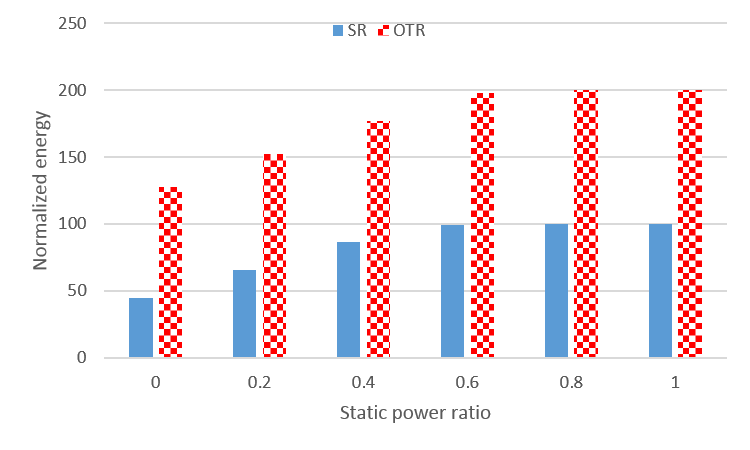
\includegraphics[width=0.45\textwidth]{figures/crash_power}
		}
		\subfigure[Sensitivity to laxity. $W=100$ hours, $\rho=0.3$, $MTBF=5$ years.]
		{
			\label{fig:crash_time}
			\includegraphics[width=0.45\textwidth]{figures/crash_time}
		}
        \subfigure[Sensitivity to workload. $\alpha=0.25$, $\rho=0.5$, $MTBF=5$ years.]
		{
			\label{fig:crash_w}
			\includegraphics[width=0.45\textwidth]{figures/crash_w}
		}
	\end{center}
	\caption{Comparison between Soft Replication and Traditional Process Replication for energy consumption under a single crash failure.}
	\label{fig:crash_eval}
\end{figure*}




\section{\uppercase{Tolerating crash failures}}
\label{sec:crash_collocation}
%In data-intensive applications, input data are divided into multiple splits that can be processed in parallel. 

To deal with crash failures, the Shadow Computing computational model can be applied, with one fast replica and one slow replica assigned to process each data partition. While each fast replica runs on one processor exclusively, multiple slow replicas could be collocated to save power and computing resources. A pair of fast and slow replicas for a partition will process the partition from two opposite ends, and complete the task by meeting in an rendezvous point. If one replica fails, however, its associated replica can continue and process the remaining data, potentially with a higher execution rate to minimize delay. Assuming at most 1 failure, the execution dynamics are depicted in Figure~\ref{fig:crash_failure_model}. %The case where both replicas fail simultaneously is ignored due to its extremely low probability. 

\begin{figure}[!t]
	\begin{center}
		\subfigure[Non-faulty task.]
		{
			\label{fig:crash1}
			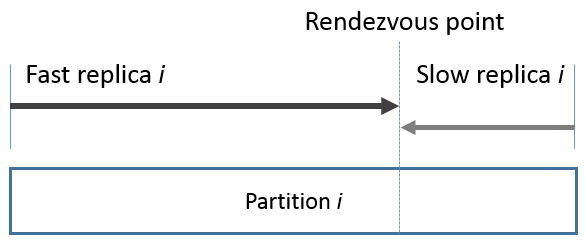
\includegraphics[width=0.9\columnwidth]{figures/crash1}
		}
		\subfigure[Fast replica failure.]
		{
			\label{fig:crash2}
			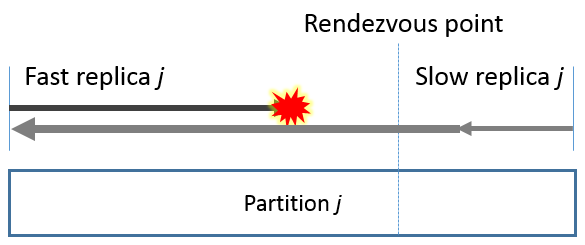
\includegraphics[width=0.9\columnwidth]{figures/crash2}
		}
        \subfigure[Slow replica failure.]
		{
			\label{fig:crash3}
			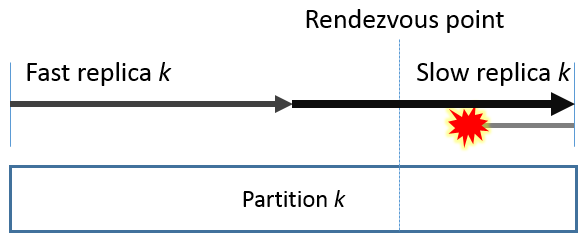
\includegraphics[width=0.9\columnwidth]{figures/crash3}
		}
	\end{center}
	\caption{Illustration of the three possible scenarios when using a pair of fast and slow replicas to process one data partition.}
	\label{fig:crash_failure_model}
\end{figure}

Note that when multiple slow replicas are collocated, to speed up one slow replica (after its associated replica fails) all the other collocated replicas need be terminated. As a result, the fast replicas associated with the terminated slow replicas also need to continue beyond the rendezvous point to process the whole partition. To facilitate the analysis of such correlation, we define \textit{shadowed set} as a set of fast replicas and their collocated slow replicas. The following subsections develop analytical models for the expected response time and energy consumption, given a failure distribution, and then formulate an optimization framework. 

\subsection{Notations}
Let $W$ denote the total amount of workload to process, and $N$ denote the number of processors available. Let $\sigma_{max}$ denote the maximal execution rate of a processor, then $R_{min}=\frac{W}{N \times \sigma_{max}}$ is the minimal response time when no failure occurs. Let $\overline{R}=(1+\alpha)R_{min}$ denote the target response time considering fault tolerance. Let $\lambda$ denote the processor failure rate, and $f(t)$ denote the failure density function. Let $E(\sigma, [t_1, t_2])$ denote the energy consumption of a processor when executing at rate $\sigma$ for an interval from $t_1$ to $t_2$.

According to the dynamics of the Soft Replication model, each processor may run at one of the following four rates:
\begin{itemize}
	\item $\sigma_{m}^{b}$, the initial rate of a processor running a fast replica
    \item $\sigma_{s}^{b}$, the initial rate of a processor running one or more slow replicas
    \item $\sigma_{m}^{a}$, the rate of a processor running a fast replica after speeding up
    \item $\sigma_{s}^{a}$, the rate of a processor running a slow replica after speeding up
\end{itemize}

\subsection{Process execution rates}
It is not difficult to derive the execution rate of each process. Since fast replicas have exclusive access to processors, their execution rates are equal to the rates of the processors that they execute on, i.e., the rate of a fast replica before/after speeding up is  $\sigma_{m}^{b}$/$\sigma_{m}^{a}$. For slow replicas, however, the execution rate depend on not only processor rate, but also on collocation ratio. Let $m$ and $n$ denote the number of processors allocated for fast and slow replicas, respectively. Collocation ratio is then derived as $m/n$, as there will be $m$ pairs of fast and slow replicas and the $m$ slow replicas will share the $n$ processors. Assuming each slow replica gets a fair share of the collocated processor's execution time, the initial rate of a slow replica is $\frac{n}{m}\sigma_{s}^{b}$. After a fast replica failure, process termination is applied so that only the slow replica associated with the failing fast replica remains. Therefore, its effective execution rate is equal to the processor rate, which is $\sigma_{s}^{a}$. 


\subsection{Response time}
\label{sec:res_time}
With a total workload of $W$ and $m$ pairs of replicas, the workload is split into $m$ ways, so the workload for each data partition is $w = W/m$.
For a shadowed set, there are three possible scenarios to consider based on the occurrence of failure, i.e., none of the processors fails, a single processor executing a fast replica fails, or a single processor executing all the slow replicas fails. The case where more than one processor fail simultaneously is ignored due to the extremely low probability.

If no processor fails, each pair of fast and slow replicas will eventually meet at the rendezvous point, which is determined by their relative execution rates. When they meet, the workload done by the fast replica plus the workload by the slow replica should be equal to $w$, and this can lead to the equation $$\sigma_m^b \times t_r^n + \frac{n}{m}\sigma_s^b \times t_r^n = w,$$ where $t_r^n$ denotes the response time when no failure occurs. Using the above equation, it is not difficult to derive that $t_r^n = \frac{w}{\sigma_m^b+\frac{n}{m}\sigma_s^b}$.

If the processor executing slow replicas fails at time $t_f$ before the rendezvous point, all fast replicas speed up to $\sigma_m^a$ and process all the remaining data in each partition. At the time of the failure, the remaining workload for each fast replica is $(w-\sigma_m^b \times t_f)$. Thus, the response time in this case can be expressed as $t_r^m = t_f + \frac{w-\sigma_m^b \times t_f}{\sigma_m^a}$.

In the last scenario, a processor executing a fast replica fails at some time, let's say $t_f$. The associated slow replica speeds up to $\sigma_s^a$ and processes all the remaining data in the partition.  At the time of the failure, the remaining workload for the slow replica is $(w-\frac{n}{m}\sigma_s^b \times t_f)$. The response time in this case can be expressed as $t_r^s = t_f + \frac{w-\frac{n}{m}\sigma_s^b \times t_f}{\sigma_s^a}$.


\subsection{Power and energy}
\label{sec:power_model}
Dynamic voltage and frequency scaling
(DVFS) is a widely available technique to reduce processor frequency. It
is well known that one can reduce the dynamic processor power consumption at
least quadratically by reducing the frequency linearly. The
dynamic processor power consumption executing at rate
$\sigma$ is given by the function $p_d(\sigma)=\sigma^n$ where $n \ge
2$. Throughout this paper we assume that dynamic power is cubic
in relation to processor frequency.

In addition to the dynamic power, processor leakage and other components
(memory, disk, network etc.) all contribute to static power
consumption, which is independent of the processor frequency. In this paper, we
define static power as a fixed fraction of the total power consumed
when executing at maximum rate, referred to as $\rho$. Hence, a processor'
power consumption is expressed as
$p(\sigma)=\rho \times \sigma_{max}^3 + (1-\rho)\times \sigma^3$. 

Using the above power model, the
energy consumed by a processor executing at rate $\sigma$ during an
interval $(t_2-t_1)$ is given by 
$E(\sigma,[t_1, t_2]) = p(\sigma) \times (t_2-t_1)$. 
Considering a shadowed set as a whole and the failure of a processor as a unit, the energy consumption also falls into three cases. Note that each shadowed set contains $m/n$ pairs of replicas, using $(m/n + 1)$ processors. 

If no failure occurs, the energy consumption of a shadowed set, weighted by its probability, is 
\begin{equation}
\begin{split}
E_1 = & (1-\int_{0}^{t_r^n} f(t)dt)^{\frac{m}{n}+1} \times \\
      & \{\frac{m}{n}E(\sigma_m^b,[0,t_r^n])+E(\sigma_s^b,[0,t_r^n])\}
%E_1 = & (1-\int_{0}^{t_r^n} f_m(t)dt)^{\frac{m}{n}} \times (1-\int_{0}^{t_r^n} f_s(t)dt) \times \\
%      & \{\frac{m}{n}E(\sigma_m^b,[0,t_r^n])+E(\sigma_s^b,[0,t_r^n])\}
\label{eq:energy_no_failure}
\end{split}
\end{equation}
The first line is the probability that none of the $m/n$ fast replica processors fails and the slow replica processor also does not fail. The second line captures the energy of all the processors in a shadowed set during the execution. 

If the slow replica processor fails, all the fast replica processors in the shadowed set will speed up. The weighted energy consumption is 
\begin{equation}
\begin{split}
E_2 = & (1-\int_{0}^{t_r^n} f(t)dt)^\frac{m}{n} \times \\
      & \int_{0}^{t_r^n} \{\frac{m}{n}E(\sigma_m^b, [0,t])+E(\sigma_s^b, [0,t]) \\       & +\frac{m}{n}E(\sigma_m^a, [t,t_r^m])\} \times f(t)dt
%E_2 = & (1-\int_{0}^{t_r^n} f_m(t)dt)^\frac{m}{n} \times \\
%      & \int_{0}^{t_r^n} \{\frac{m}{n}E(\sigma_m^b, [0,t])+E(\sigma_s^b, [0,t]) \\       & +\frac{m}{n}E(\sigma_m^a, [t,t_r^m])\} \times f_s(t)dt
\end{split}
\end{equation}   
The energy contains the part of all the processors before the failure, and that of the fast replica processors executing at a higher rate until the completion. 

If a fast replica processor fails, the slow replica processor and all remaining fast replica processors speed up. The weighted energy consumption is 
\begin{equation}
\begin{split}
E_3 = & \frac{m}{n} \times (1-\int_{0}^{t_r^n} f(t)dt)^{\frac{m}{n}}  \times \\
      & \int_{0}^{t_r^n} \{\frac{m}{n} \times E(\sigma_m^b, [0,t]) + (\frac{m}{n}-1)E(\sigma_m^a,[t, t_r^m]) + \\ 
      & +E(\sigma_s^b, [0,t])+E(\sigma_s^a, [t,t_r^s])\} \times f(t)dt
%E_3 = & \frac{m}{n}(1-\int_{0}^{t_r^n} f_m(t)dt)^{\frac{m}{n}-1} \times (1-\int_{0}^{t_r^n} f_s(t)dt) \times \\
%      & \int_{0}^{t_r^n} \{\frac{m}{n} \times E(\sigma_m^b, [0,t]) + (\frac{m}{n}-1)E(\sigma_m^a,[t, t_r^m]) + \\ 
%      & +E(\sigma_s^b, [0,t])+E(\sigma_s^a, [t,t_r^s])\} \times f_m(t)dt
\end{split}
\end{equation}  
The factor of $\frac{m}{n}$ in the probability reflects the possibility that any of the fast replica processors may fail. In addition to the energy consumed before the failure, the above equation also calculates the energy of the remaining processors after speeding up. 

The total energy consumption of the entire job is the sum of the above three, multiplied by the number of shadowed set, i.e., $E_{total}=n \times (E_1+E_2+E_3)$.

\subsection{Shadowed set vulnerability}
As a side effect of collocation, each shadowed set can only tolerate one crash failure, and a second failure will result in a re-execution.  If a second failure in a shadowed set occurs, this situation is referred to as a \textit{shadowed set failure}. It is not difficult to see that the probability of such case depends on the number of processors in each shadowed set and the failure likelihood of each processor. The following part models the shadowed set failure probability. 

Given the response time calculated in above section, the probability of a processor failure during a job's execution is $\int_{0}^{t_r^n} f(t)dt$. For a shadowed set with $\frac{m}{n}+1$ processors, the probability that no processor fails is $P_0=(1-\int_{0}^{t_r^n} f(t)dt)^{\frac{m}{n}+1}$, and the probability that there is exactly one failure is $P_1 = (\frac{m}{n}+1) \times \int_{0}^{t_r^n} f(t)dt \times (1-\int_{0}^{t_r^n} f(t)dt)^{\frac{m}{n}}$.
Since there need to be at least two failures for a shadowed set to fail. the shadowed set failure probability is $P_{set} = 1 - P_0 - P_1$. 


\subsection{Optimization}
\label{sec:crash_opt}
An optimization problem can be formulated to derive the optimal execution rates for both the fast and slow replicas, as well as the optimal collocation ratio for the slow replicas, given an objective and constraint(s). Below we show a case study that minimizes the total energy consumption while meeting response time constraint. 

\begin{equation}
\begin{alignedat}{2}
\min_{\sigma_m^b,\sigma_s^b,\sigma_m^a,\sigma_s^a, m, n} \qquad  & E_{total}(W,N,\overline{R},\rho,\lambda,\sigma_{max},F_t) \\
s.t.  \qquad          & 0 \leq \sigma_m^b \leq \sigma_{max} \\
                      & 0 \leq \frac{n}{m}\sigma_s^b \leq \sigma_m^b \\
                     & \sigma_m^b \leq \sigma_m^a \leq \sigma_{max} \\
                     & \frac{n}{m}\sigma_s^b \leq \sigma_s^a \leq \sigma_{max} \\
                     & 1 \leq n \leq m \leq N \\
                      & max(t_r^n, t_r^m, t_r^s) \leq \overline{R} \\
                      & P_{set} < F_t
\end{alignedat}
\end{equation}

The first constraint says the initial rate of a fast replica should observe the physical processor limit. The second constraint indicates that the initial rate of a slow replica should not exceed that of a fast replica. The third and fourth constraints ensure that fast and slow replicas could speed up after detecting a failure. The next constraint guarantees that the deadline is met even in the presence of failure. Although $t_r^m$ and $t_r^s$ depend on the failure occurrence time, it is clear that the most demanding condition is that if failure occurs at the last moment before reaching the rendezvous point, the remaining replica can still process the entire partition before the deadline. The last constraint can be applied if there is a desire for a threshold on the probability that the job needs to be re-executed.

%\section{\uppercase{Dealing with silent data corruption}}
%\label{sec:silent}
%%\section{Dealing with silent data corruption}
Different from crash failures, which crashes a process, silent data corruption allows a faulty process to continue to completion but generate incorrect results. To deal with $f$ failures of this type, $(2f+1)$ replicas are needed, and voting is involved at the end to identify the correct results. For example, when at most 1 silent data corruption could occur, 3 replicas are necessary and sufficient to tolerate the failure. In the following, we will focus on tolerating one silent data corruption per data split. 

Soft Replication can deal with silent data corruption with potentially higher efficiency and less resource requirement compared to traditional replication techniques. For each split, Soft Replication associates 2 fast replicas with 1 slow replica. To save energy, the slow replica executes at a potentially lower rate than the 2 fast replicas, and dynamically speeds up if a fast replica fails. 

\subsection{Notations}
Let $W$ denote the required workload to process one data split, which is often the unit of transfer from disk to main memory. Let $\sigma_{max}$ denote the maximal execution rate, then $R_{min}=\frac{W}{\sigma_{max}}$ is the minimal response time. Let $\overline{R}=(1+\alpha)R_{min}$ $(0\leq \alpha \leq 1)$ denote the fault-tolerant response time. Let $\lambda$ denote the failure rate, and $f(t)$ denote the failure density function. Let $E(\sigma, [t_1, t_2])$ denote the energy consumption of a process when executing at rate $\sigma$ for an interval from $t_1$ to $t_2$.

To deal with silent data corruption, the Soft Replication model entails three execution rates:
\begin{itemize}
	\item $\sigma_{m}$, the execution rate of the fast replicas 
    \item $\sigma_{b}$, the execution rate of the slow replica before a fast replica fails
    \item $\sigma_{a}$, the execution rate of the slow replica after a fast replica fails
\end{itemize}

\subsection{Response time}
Assuming there is at most one silent data corruption, three scenarios need to be considered, i.e., no failure, one fast replica fails, or the slow replica  fails.

In the first scenario, where no failure occurs, the response time is determined by the fast replicas, as $t_r^m=\frac{W}{\sigma_m}$.

In the second scenario, 
where the slow replica fails, the fast replicas are not impacted, and thus the response time is also determined by the fast replicas, as in the first scenario. Therefore, $t_r^m=\frac{W}{\sigma_m}$.


In the last scenario, where one fast replica fails, the response time is determined by the slow replica. The work completed by the slow replica before the fast replicas complete is $w_b = \sigma_b \times t_r^m$. Then the remaining work for the slow replica to complete is $w_a = W - w_b$. As a result, the total response time by the slow replica is $t_r^s = t_r^m + \frac{w_a}{\sigma_a} = \frac{W(\sigma_m + \sigma_a - \sigma_b)}{\sigma_m \sigma_a}$.



\subsection{Energy consumption}
To calculate energy consumption, we also use the power model described in Section~\ref{sec:power_model}.
Corresponding to the three scenarios in the above response time analysis, the energy consumption also falls into three cases. 

If no failure occurs, the energy consumption of the three replicas weighted by its probability is
\begin{equation}
\begin{split}
E_1 = & (1 - \int_{0}^{t_r^m} f_m(t)dt)^2 \times (1 - \int_{0}^{t_r^m} f_s(t)dt) \times \\
      & \{2E(\sigma_m, [0, t_r^m])+E(\sigma_b, [0, t_r^m])\}
\end{split}
\end{equation}

If one fast replica fails, the energy consumption weighted by its probability is 
\begin{equation}
\begin{split}
E_2 = & 2(1 - \int_{0}^{t_r^m} f_m(t)dt) \times 
(1 - \int_{0}^{t_r^m} f_s(t)dt) \times \int_{0}^{t_r^m} f_m(t)dt \times \\       & \{2E(\sigma_m, [0, t_r^m]) + E(\sigma_b, [0, t_r^m]) + E(\sigma_a, [t_r^m, t_r^s])  \}
\end{split}
\end{equation}

If the slow replica fails, the energy consumption weighted by its probability is 
\begin{equation}
\begin{split}
E_3 = & (1 - \int_{0}^{t_r^m} f_m(t)dt)^2 \times \int_{0}^{t_r^m} f_s(t)dt \times \\  & \{2E(\sigma_m, [0, t_r^m])+E(\sigma_b, [0, t_r^m])\}
\end{split}
\end{equation}

All in all, the total energy consumption is the sum of the above three, i.e., $E_{total}=E_1 + E_2 + E_3$. 

\subsection{Optimization}
Similar to dealing with crash failures, an optimization problem can be formulated for dealing with silent data corruption to derive the optimal values for the three execution rates, in order to minimize the total energy consumption while meeting response time constraint. 

\begin{equation}
\begin{alignedat}{2}
\min_{\sigma_m,\sigma_b,\sigma_a} \qquad  & E_{total} \\
s.t.  \qquad          & 0 \leq \sigma_m \leq \sigma_{max} \\
                      & 0 \leq \sigma_b \leq \sigma_m \\
                      & \sigma_b \leq \sigma_a \leq \sigma_{max} \\
                      & max(t_r^m, t_r^s) \leq \overline{R}
\end{alignedat}
\end{equation}

The first constraint says the execution rate of the fast replicas should observe the physical processor limit. The second constraint indicates that the slow replica should not exceed the execution rate of the fast replicas. The third constraint ensures that the slow replica could speed up after detecting a failure. The last constraint guarantees that the deadline is met even in the case of failure.



\subsection{Performance evaluation}

\begin{figure*}[!t]
	\begin{center}
		\subfigure[Sensitivity to failure rate. $W=100$ hours, $\alpha=0.25$, $\rho=0.5$.]
		{
			\label{fig:silent_lambda}
			\includegraphics[width=0.45\textwidth]{figures/silent_lambda}
		}
		\subfigure[Sensitivity to static power ratio. $W=100$ hours, $\alpha=0.25$, $MTBF=5$ years.]
		{
			\label{fig:silent_power}
			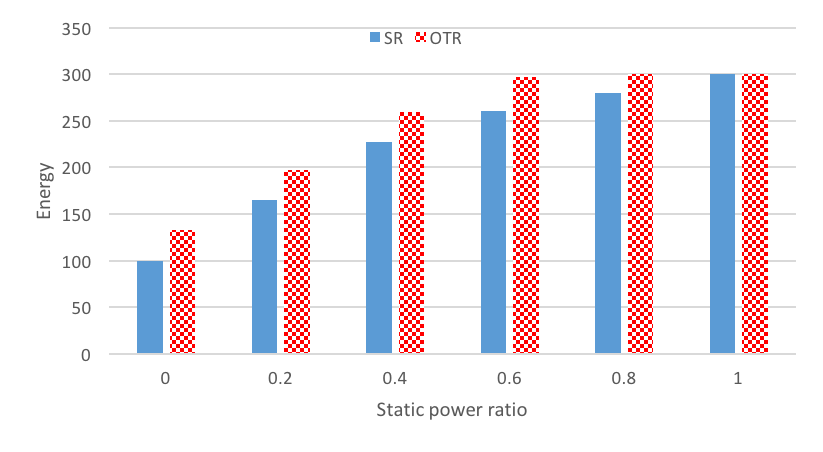
\includegraphics[width=0.45\textwidth]{figures/silent_power}
		}
		\subfigure[Sensitivity to laxity. $W=100$ hours, $\rho=0.3$, $MTBF=5$ years.]
		{
			\label{fig:silent_time}
			\includegraphics[width=0.45\textwidth]{figures/silent_time}
		}
        \subfigure[Sensitivity to workload. $\alpha=0.25$, $\rho=0.5$, $MTBF=5$ years.]
		{
			\label{fig:silent_w}
			\includegraphics[width=0.45\textwidth]{figures/silent_w}
		}
	\end{center}
	\caption{Comparison between Soft Replication and Traditional Process Replication for energy consumption under a single silent failure.}
	\label{fig:silent_eval}
\end{figure*}






%\section{\uppercase{Dealing with silent data corruption (adding checkpoints)}}
%\label{sec:silent_cp}
%%\section{Dealing with silent data corruption}
Different from crash failures, which crashes a process, silent data corruption allows a faulty process to continue to completion but generate incorrect results. To deal with $f$ failures of this type, $(2f+1)$ replicas are needed, and voting is involved at periodic checkpoints to detect failure. For example, when at most 1 silent data corruption could occur, 3 replicas are necessary and sufficient to tolerate the failure. In the following, we will focus on tolerating one silent data corruption per data split. 

Soft Replication can deal with silent data corruption with potentially higher efficiency and less resource requirement compared to traditional replication techniques. For each split, Soft Replication associates 2 fast replicas with 1 slow replica. To save energy, the slow replica executes at a potentially lower rate than the 2 fast replicas, and dynamically speeds up if a fast replica fails. 

\subsection{Notations}
Let $W$ denote the required workload to process one data split, which is often the unit of transfer from disk to main memory. Let $w$ denote the checkpoint interval. The number of checkpoints is $\frac{W}{w}$. Let $\sigma_{max}$ denote the maximum execution rate. $R_{min}=\frac{W}{\sigma_{max}}$ is the minimal response time. Let $\overline{R}=(1+\alpha)R_{min}$ $(0\leq \alpha \leq 1)$ denote the fault-tolerant response time. Let $\lambda$ denote the failure rate, and $f(t)$ denote the failure density function. Let $E(\sigma, [t_1, t_2])$ denote the energy consumption of a process when executing at rate $\sigma$ for an interval from $t_1$ to $t_2$.

To deal with silent data corruption, the Soft Replication model entails four execution rates:
\begin{itemize}
	\item $\sigma_{m}^b$, the execution rate of the fast replicas before a slow replica fails
    \item $\sigma_{m}^a$, the execution rate of the fast replicas after a slow replica fails
    \item $\sigma_{s}^b$, the execution rate of the slow replica before a fast replica fails
    \item $\sigma_{s}^a$, the execution rate of the slow replica after a fast replica fails
\end{itemize}

\subsection{Response time}
Assuming there is at most one silent data corruption, three scenarios need to be considered, i.e., no failure, one fast replica fails, or the slow replica  fails.

In the first scenario, where no failure occurs, the response time is determined by the fast replicas, as $t_r^n=\frac{W}{\sigma_{m}^b}$.

In the second scenario, 
where the slow replica fails, only one fast replica needs to keep running after detecting this failure, and the fast replica can potentially slow down because there will be no more failures.
%the fast replicas are not impacted, and thus the response time is also determined by the fast replicas, as in the first scenario. Therefore, $t_r^m=\frac{W}{\sigma_m}$.
The failure detection time depends on the failure occurrence time. The current checkpoint interval index for the slow replica is $\left \lceil{\frac{t_f \times \sigma_s^b}{w}}\right \rceil$. The detection time is $d_s(t_f) = \left \lceil{\frac{t_f \times \sigma_s^b}{w}}\right \rceil \times \frac{w}{\sigma_s^b}$. The response time is $t_r^m = d_s(t_f) + \frac{W - d_s(t_f)\times \sigma_m^b}{\sigma_m^a}$. 

In the last scenario, where one fast replica fails, both fast replicas can be terminated after detecting the failure and the remaining slow replica may speed up. The current checkpoint interval index for the fast replicas is $\left \lceil{\frac{t_f \times \sigma_m^b}{w}}\right \rceil$. The detection time is $d_m(t_f) = \left \lceil{\frac{t_f \times \sigma_m^b}{w}}\right \rceil \times \frac{w}{\sigma_m^b}$. The response time is $t_r^s = d_m(t_f) + \frac{W - d_m(t_f)\times \sigma_s^b}{\sigma_s^a}$. 
%the response time is determined by the slow replica. The work completed by the slow replica before the fast replicas complete is $w_b = \sigma_b \times t_r^m$. Then the remaining work for the slow replica to complete is $w_a = W - w_b$. As a result, the total response time by the slow replica is $t_r^s = t_r^m + \frac{w_a}{\sigma_a} = \frac{W(\sigma_m + \sigma_a - \sigma_b)}{\sigma_m \sigma_a}$.



\subsection{Energy consumption}
To calculate energy consumption, we also use the power model described in Section~\ref{sec:power_model}.
Corresponding to the three scenarios in the above response time analysis, the energy consumption also falls into three cases. 

If no failure occurs, the energy consumption of the three replicas weighted by its probability is
\begin{equation}
\begin{split}
E_1 = & (1 - \int_{0}^{t_r^n} f_m(t)dt)^2 \times (1 - \int_{0}^{t_r^n} f_s(t)dt) \times \\
      & \{2E(\sigma_m^b, [0, t_r^n])+E(\sigma_s^b, [0, t_r^n])\}
\end{split}
\end{equation}

If one fast replica fails, the energy consumption weighted by its probability is 
\begin{equation}
\begin{split}
E_2 = & 2(1 - \int_{0}^{t_r^n} f_m(t)dt) \times 
(1 - \int_{0}^{t_r^n} f_s(t)dt) \\ \times  & \int_{0}^{t_r^n}                \{2E(\sigma_m^b, [0, d_m(t)]) + E(\sigma_s^b, [0,  d_m(t)])  \\
& + E(\sigma_s^a, [d_m(t), t_r^s])  \} \times  f_m(t)dt
\end{split}
\end{equation}

If the slow replica fails, the energy consumption weighted by its probability is 
\begin{equation}
\begin{split}
E_3 = & (1 - \int_{0}^{t_r^n} f_m(t)dt)^2 \times   \\  & \int_{0}^{t_r^n} \{2E(\sigma_m^b, [0, d_s(t)])+E(\sigma_s^b, [0, d_s(t)]) \\ & + E(\sigma_m^a, [d_s(t)], t_r^m)\} \times f_s(t)dt 
\end{split}
\end{equation}

All in all, the total energy consumption is the sum of the above three, i.e., $E_{total}=E_1 + E_2 + E_3$. 

\subsection{Optimization}
Similar to dealing with crash failures, an optimization problem can be formulated for dealing with silent data corruption to derive the optimal values for the four execution rates, in order to minimize the total energy consumption while meeting response time constraint. 

\begin{equation}
\begin{alignedat}{2}
\min_{\sigma_m^b,\sigma_m^a,\sigma_s^b,\sigma_s^a} \qquad  & E_{total} \\
s.t.  \qquad          & 0 \leq \sigma_m^b \leq \sigma_{max} \\
					  & 0 \leq \sigma_m^a \leq \sigma_m^b \\
                      & 0 \leq \sigma_s^b \leq \sigma_m^b \\
                      & \sigma_s^b \leq \sigma_s^a \leq \sigma_{max} \\
                      & max(t_r^n,t_r^m, t_r^s) \leq \overline{R}
\end{alignedat}
\end{equation}

The first constraint says the execution rate of the fast replicas should observe the physical processor limit. The second constraint indicates that the slow replica should not exceed the execution rate of the fast replicas. The third constraint ensures that the slow replica could speed up after detecting a failure. The last constraint guarantees that the deadline is met even in the case of failure.



\subsection{Performance evaluation}

\begin{figure*}[!t]
	\begin{center}
		\subfigure[Sensitivity to failure rate. $W=100$ hours, $\alpha=0.25$, $\rho=0.5$.]
		{
			\label{fig:silent_lambda}
			\includegraphics[width=0.45\textwidth]{figures/silent_lambda}
		}
		\subfigure[Sensitivity to static power ratio. $W=100$ hours, $\alpha=0.25$, $MTBF=5$ years.]
		{
			\label{fig:silent_power}
			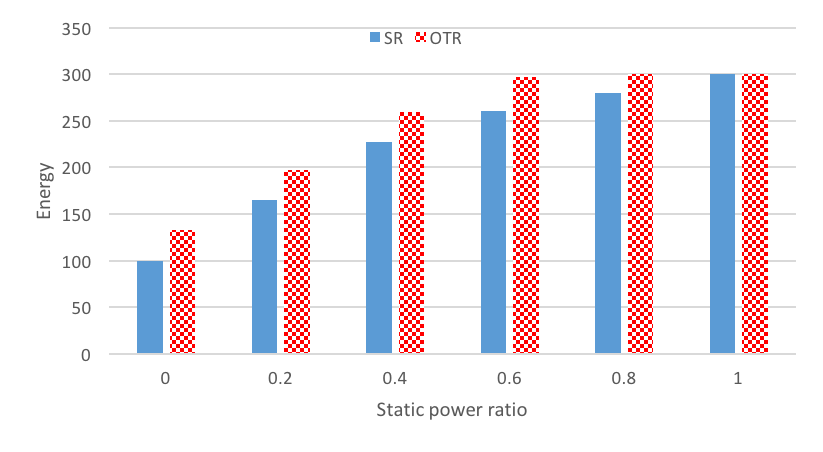
\includegraphics[width=0.45\textwidth]{figures/silent_power}
		}
		\subfigure[Sensitivity to laxity. $W=100$ hours, $\rho=0.3$, $MTBF=5$ years.]
		{
			\label{fig:silent_time}
			\includegraphics[width=0.45\textwidth]{figures/silent_time}
		}
        \subfigure[Sensitivity to workload. $\alpha=0.25$, $\rho=0.5$, $MTBF=5$ years.]
		{
			\label{fig:silent_w}
			\includegraphics[width=0.45\textwidth]{figures/silent_w}
		}
	\end{center}
	\caption{Comparison between Soft Replication and Traditional Process Replication for energy consumption under a single silent failure.}
	\label{fig:silent_eval}
\end{figure*}






\section{\uppercase{Tolerating silent data corruption}}
\label{sec:silent_cp_leap}
%\section{Dealing with silent data corruption}
Different from crash failures which crashes a processor, silent data corruption allows a faulty processor to continue to completion but may silently generate incorrect results. To deal with $f$ failures, $(2f+1)$ replicas are needed, and voting is required periodically to detect failure. For example, when at most 1 silent data corruption could occur, 3 replicas are sufficient to detect and tolerate the failure. In the following, we will focus on tolerating one silent data corruption per data partition. 

Compared to traditional replication techniques, Shadow Computing can deal with silent data corruption with higher efficiency and less resource requirement. For each partition, Shadow Computing associates 2 fast replicas with 1 slow replica. To save energy, the slow replica executes at a potentially lower rate than the 2 fast replicas, and dynamically speeds up if a fast replica fails. 

To take advantage of the fast progress of the fast replicas, Shadow Computing could perform a leaping at a voting point to leap forward the slow replica. Specifically, when two fast replicas reach a voting point with agreement, the results and execution state are copied to the slow replica to achieve forward progress. This is illustrated in Figure~\ref{fig:silent_model}. If one fast replica fails, the failure will be detected at the next voting point. At this time, the slow replica speeds up to reach the specific voting point and participate in the voting to detect the failed replica. Then a leaping from one correct replica to the failed replica can rejuvenate the failed one, after which all replicas resume normal execution. Note that the slow replica is only useful when one of the fast replicas fails. If the slow replica fails, it will automatically get rejuvenated when the fast replicas reach the next voting point. 

\begin{figure}[!t]
  \begin{center}
      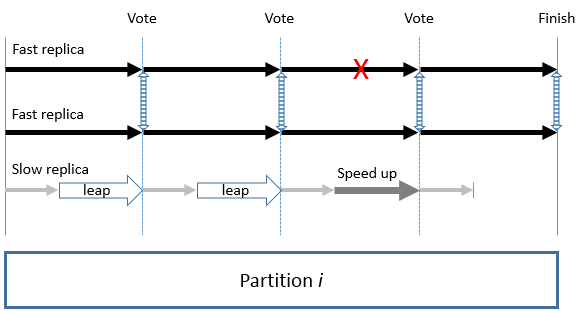
\includegraphics[width=\columnwidth]{figures/silent_model}
  \end{center}
  \vskip -0.1in
  \caption{Tolerating silent data corruption by using two fast replicas with one slow replica.}
  \label{fig:silent_model}
  %\vspace{-0.05in}
\end{figure}

Similar to Section~\ref{sec:crash_collocation}, following subsections develop analytical models for the expected response time and energy consumption, and formulate an optimization framework. (!Explain why didn't consider collocation)

\subsection{Notations}
Let $W$ denote the required workload to process one partition. Let $N$ denote the number of voting points. The voting interval is $w=\frac{W}{N}$. Let $\sigma_{max}$ denote the maximum execution rate. $R_{min}=\frac{W}{\sigma_{max}}$ is the minimal response time. Let $\overline{R}=(1+\alpha)R_{min}$ $(0\leq \alpha \leq 1)$ denote the target response time considering fault tolerance. Let $\lambda$ denote the failure rate, and $f(t)$ denote the failure density function. %Let $d(t)$ denote the failure detection time at a voting point. 
Let $E(\sigma, [t_1, t_2])$ denote the energy consumption of a replica when executing at rate $\sigma$ for an interval from $t_1$ to $t_2$. For each leaping, let $T_l$ denote the time cost, and $E_l$ denote the energy cost.

To deal with silent data corruption, the Shadow Computing model entails three execution rates:
\begin{itemize}
	\item $\sigma_m$, the execution rate of the fast replicas 
    \item $\sigma_b$, the execution rate of the slow replica before a fast replica fails
    \item $\sigma_a$, the execution rate of the slow replica after a fast replica fails
\end{itemize}

\subsection{Response time}
Assuming there is at most one silent data corruption, two scenarios need to be considered, i.e., no fast replica failure, or one fast replica fails. The failure of the slow replica has no impact on the response time. 

In the first scenario, where no failure occurs, the execution time is determined by the fast replicas, as $t_r^m=\frac{W}{\sigma_m}$. Considering the time for leaping, the total response time is $t_{rl}^m=\frac{W}{\sigma_m} + N \times T_l$.

In the second scenario, 
where a fast replica fails, the delay is the time for the slow replica to catch up with respect to a voting interval. The time for a fast replica to complete a voting interval is $t_v = \frac{w}{\sigma_m}$. The time required by the slow replica to complete the remaining work in the current interval is $t_d = \frac{w - t_v\times \sigma_b}{\sigma_a}$. The execution time is $t_r^s = t_r^m + t_d$. Considering the time for leaping, the total response time is $t_{rl}^s=t_r^s + N \times T_l$.
%the response time is determined by the slow replica. The work completed by the slow replica before the fast replicas complete is $w_b = \sigma_b \times t_r^m$. Then the remaining work for the slow replica to complete is $w_a = W - w_b$. As a result, the total response time by the slow replica is $t_r^s = t_r^m + \frac{w_a}{\sigma_a} = \frac{W(\sigma_m + \sigma_a - \sigma_b)}{\sigma_m \sigma_a}$.



\subsection{Energy consumption}
To calculate energy consumption, we also use the power model described in Section~\ref{sec:power_model}.
Corresponding to the two scenarios in the above response time analysis, the energy consumption also falls into two cases. 

If neither of the fast replicas fails, the energy consumption of the three replicas weighted by its probability is
\begin{equation}
\begin{split}
E_1 = & (1 - \int_{0}^{t_r^m} f(t)dt)^2  \times \\
      & \{2E(\sigma_m, [0, t_r^m])+E(\sigma_b, [0, t_r^m])\}
%E_1 = & (1 - \int_{0}^{t_r^m} f_m(t)dt)^2  \times \\
%      & \{2E(\sigma_m, [0, t_r^m])+E(\sigma_b, [0, t_r^m])\}
\end{split}
\end{equation}
The first line is the probability that neither of the fast replicas fails. The second line models the energy of the three replicas during normal execution.

If one fast replica fails, the energy consumption weighted by its probability is 
\begin{equation}
\begin{split}
E_2 = & 2(1 - \int_{0}^{t_r^m} f(t)dt) \times \int_{0}^{t_r^m} f(t)dt \times 
\\  & \{2E(\sigma_m, [0, t_r^m])+E(\sigma_b, [0, t_r^m]) \\ & + 2E(0, [t_r^m, t_r^s])+E(\sigma_a, [t_r^m, t_r^s]\} 
%E_2 = & 2(1 - \int_{0}^{t_r^m} f_m(t)dt) \times \int_{0}^{t_r^m} f_m(t)dt \times 
%\\  & \{2E(\sigma_m, [0, t_r^m])+E(\sigma_b, [0, t_r^m]) \\ & + 2E(0, [t_r^m, t_r^s])+E(\sigma_a, [t_r^m, t_r^s]\} 
\end{split}
\end{equation}
The first line calculates the probability that one fast replica fails while the other successfully completes. In addition to the energy in the first scenario, also accounted is the energy consumed during slow replica catches up, including the fast replicas' idly waiting and the slow replica's speeding up. 



All in all, the total energy consumption is the sum of the above two, plus the energy cost of leaping, i.e., $E_{total}=E_1 + E_2 + N\times E_l$. 

\subsection{Optimization}
\label{sec:silent_opt}
Similar to dealing with crash failures, an optimization problem can be formulated for dealing with silent data corruption to derive the optimal values for the three execution rates, in order to minimize the total energy consumption while meeting response time constraint. 

\begin{equation}
\begin{alignedat}{2}
\min_{\sigma_m,\sigma_s^b,\sigma_s^a} \qquad  & E_{total} (W,N,\overline{R},\rho,\lambda,\sigma_{max}, T_l, E_l)  \\
s.t.  \qquad          & 0 \leq \sigma_m \leq \sigma_{max} \\
                      & 0 \leq \sigma_s^b \leq \sigma_m\\
                      & \sigma_s^b \leq \sigma_s^a \leq \sigma_{max} \\
                      & t_{rl}^s \leq \overline{R}
\end{alignedat}
\end{equation}

The first constraint says the execution rate of the fast replicas should observe the physical processor limit. The second constraint indicates that the initial rate of the slow replica should not exceed that of the fast replicas. The third constraint ensures that the slow replica could speed up after detecting a failure. The last constraint guarantees that the deadline is met even in the case of failure.









\section{\uppercase{Evaluation}}
\label{sec:eval}
Extensive experiments have been done to validate our design of VTC as well as evaluate 
its performance under various scenarios. This section covers our testbeds, experiment 
methodologies, performance tuning, results, and analysis. 

\subsection{Experiment setup}
The experiments are conducted in two phases. In the first phase, only CPU is over-committed 
to validate the design of VTC with over-commitment. In this phase, we used a cluster of 18 nodes (1 login node, 1 management node, and 16 compute nodes) to mimic a realistic HPC computing environment. Each node has dual 10-core Intel Xeon E5-2660 processor and 128 GB DDR4 memory. %, and 10 Gb Ethernet. 
The hypervisor used is VMware ESXi 6.5, OS is CentOS 7.3, and resource manager is TORQUE 6.1 with the default job scheduler. We use compute-intensive benchmarks from PolyBench/C 3.1 and BioPerf~\cite{1526013}. 
In the second phase, we evaluate the full-fledged VTC design with both CPU and memory over-commitment on another testbed with huge memory capacity for memory-intensive workloads. The second cluster has 1 login, 1 management, and 8 compute nodes. Each node has dual 16-core Intel Xeon Gold 6130 processor and 768 GB memory. %, and 10 Gb Ethernet. 
The hypervisor used is VMware ESXi 6.7, OS is CentOS 7.6, and resource manager is TORQUE 6.1 with the default job scheduler. We add memory-intensive benchmarks from HPCC~\cite{dongarra2004introduction}.

\subsection{CPU over-commitment}
For performance evaluation, each node is installed with two execution environments on two separate booting disks, that is, a native OS and an ESXi hypervisor. With the hypervisor, we further define three VTC scenarios: 1) one virtual cluster; 2) two virtual clusters; 3) four virtual clusters. The latter two scenarios have 2X and 4X CPU over-commitment, respectively. 
When comparing performance among different execution scenarios (including bare metal cluster), we run the same job stream which consists of 3248 jobs that are randomly sampled from the PolyBench and BioPerf suites, and the wall clock execution time is shown in Figure~\ref{fig:cpu_exe_time}.

\begin{figure}[!t]
   \begin{center}
       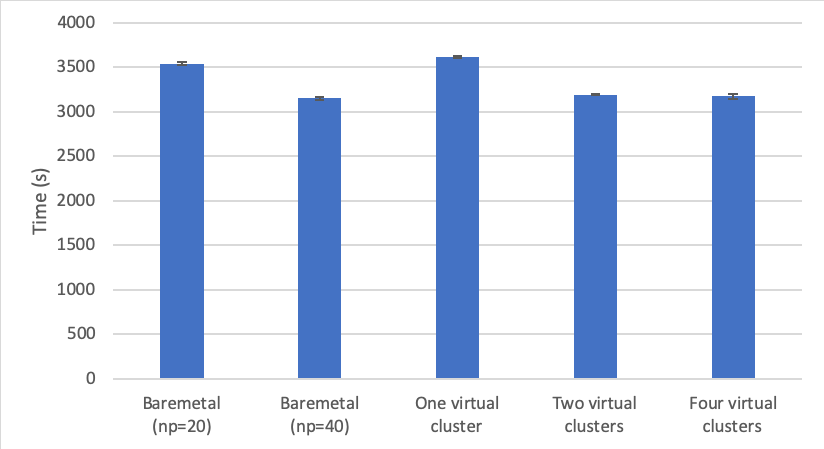
\includegraphics[width=\columnwidth]{Figures/cpu_exe_time}
   \end{center}
   \caption{Comparison of wall clock execution time for a job stream between bare metal and VTC with different CPU over-commitment ratios. Results are average of three runs.}
   \label{fig:cpu_exe_time}
 \end{figure}

Because each node in our testbed has 20 cores, in the first experiment we configured each TORQUE worker with 20 job slots. As reflected in Figure~\ref{fig:cpu_exe_time}, the execution with one virtual cluster is very close to that of bare metal (first column), with only a 2.2 percent overhead. Furthermore, when multiple virtual clusters are used with CPU over-commitment, the execution time is surprisingly shorter, implying an improved throughput despite the virtualization overhead. Through careful analysis, we identified that the throughput improvement can mainly be attributed to increased CPU utilization when more jobs are concurrently scheduled to execute. This has been verified by modifying each TORQUE worker in the bare-metal environment to use 40 job slots, after which the throughput is improved to the same level as the over-committed virtual environment. This can be seen in the second column of Figure~\ref{fig:cpu_exe_time}.

Besides execution time, another performance metric that we monitored is the total CPU utilization across the whole cluster. On the ESXi hypervisor, we used esxtop running on each compute node to sample CPU utilization of all VMs at 5-second intervals, and the results for one, two, and four virtual clusters are shown in Figure~\ref{fig:cpu_utilizations}. With two and four virtual clusters, the decreasing trend at the end is due to job completion. Clearly, CPU utilization is consistent with the job execution times in Figure~\ref{fig:cpu_exe_time}. For example, the lowest CPU utilization case--one virtual cluster--matches the longest job execution time. The higher CPU utilization with two and four virtual clusters is due to resource consolidation brought about by virtualization. That is, when multiple virtual clusters share a physical cluster, the CPU scheduler on each ESXi host has more jobs to schedule and is therefore able to make better scheduling decisions by taking advantage of Hyper-Threading and eliminating idle cycles. At the same time, improved utilization comes with better consistency, where the utilization with two and four virtual clusters is much smoother than in the single-cluster case.

\begin{figure}[!t]
   \begin{center}
       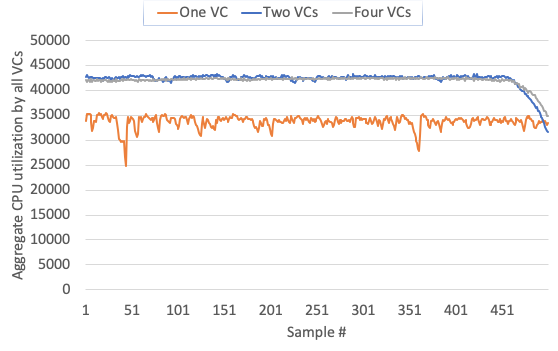
\includegraphics[width=\columnwidth]{Figures/cpu_utilizations}
   \end{center}
   \caption{Aggregate CPU utilization across 16 nodes at 5-seconds intervals.}
   \label{fig:cpu_utilizations}
   \vspace{-0.2in}
 \end{figure}

 In a production cloud environment, an important principle is fairness when multiple tenants are sharing the computing resources. We further examined the per-cluster CPU utilization in the multiple-cluster cases, and the case of four virtual clusters is shown in Figure~\ref{fig:per_cluster_utilization}. It is clear that the ESXi scheduler effectively maintains fairness so that each virtual cluster gets the same amount of CPU resources. The case of two virtual clusters is 
 the same thus not discussed. 


\begin{figure}[!t]
   \begin{center}
       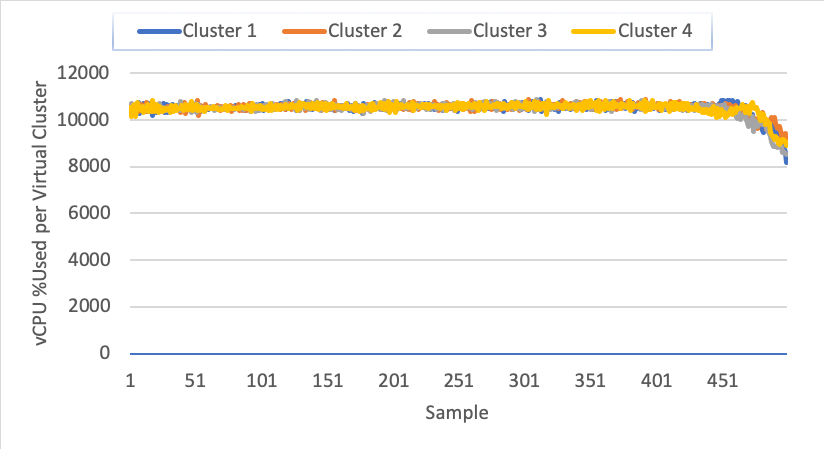
\includegraphics[width=\columnwidth]{Figures/per_cluster_utilization}
   \end{center}
   \caption{Plot of CPU utilization per virtual cluster at 5-seconds intervals for fairness check.}
   \label{fig:per_cluster_utilization}
   \vspace{-0.2in}
 \end{figure}

\subsection{CPU over-commitment with shares}
In addition to the option of equally sharing resources, the proportional, share-based scheduler of the ESXi hypervisor offers a very useful degree of flexibility. This subsection continues the CPU over-commitment study by configuring virtual clusters with different shares, to demonstrate the capability of creating a multi-tenant environment with quality-of-service guarantees. 

With the use of CPU shares, each VM can be given a particular guaranteed share of CPU resources. When there are multiple VMs running on an ESXi host, the ESXi scheduler allocates CPU based on the ratio of shares among all the running VMs. This feature extends to a virtualized HPC cloud. Specifically, each user or group can be given an appropriate share of the physical system when their virtual cluster is allocated. In this experiment, we focus on the case of four virtual clusters and set the shares ratio among the four VMs as 2:1:1:1 on every compute node. The CPU utilization is shown in Figure~\ref{fig:share_utilization}. Clearly, the CPU utilization ratio among the virtual clusters is the same as the specified shares ratio. Another important observation is that the aggregate CPU utilization across 4 virtual clusters is the same as previous no-shares case as depicted in Figure~\ref{fig:cpu_utilizations}.


\begin{figure}[!t]
   \begin{center}
       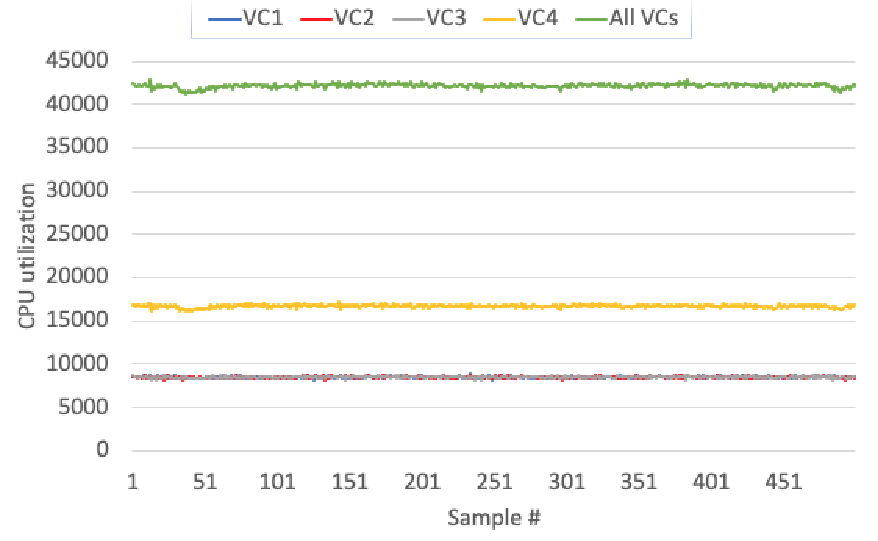
\includegraphics[width=\columnwidth]{Figures/share_utilization}
   \end{center}
   \caption{CPU utilization for four virtual clusters with 2:1:1:1 CPU shares. Utilization is sampled at 5-second intervals.}
   \label{fig:share_utilization}
 \end{figure}

\subsection{CPU + memory over-commitment}
Given that memory over-commitment is more challenging, we only test two virtual clusters with 2X CPU and memory over-commitment. vSphere Dynamic Resource Scheduler (DRS) is used to dynamically control VM migration for load balancing~\cite{infrastructure2006resource}. Considering the VM migration cost, we decided to use four quarter-size VMs to replace the single full-size VM on each node for each tenant. As a result, each tenant in this experiment gets a virtual cluster of 32 VMs across the 8 node cluster. 

To stress the system memory, we added benchmarks from HPCC. For all these HPCC benchmarks, a problem size of 53664 is chosen to have the memory consumption ranging from 16 GB to 22 GB per job instance. All the benchmarks are run with a single threaded process to mimic throughput workloads. 
To model a real HPC tenant, we specify the job arrival time to follow a Gamma distribution based on the study of several production HPC systems~\cite{lublin2003workload}.  
The resulted mean job inter-arrival time is 20.88 seconds
%The Gamma distribution has a shape parameter of 10.23 and scale parameter of 0.49. With those parameters, the mean job inter-arrival time is 10.23 / 0.49 = 20.88 seconds. 
%Also, all job sequences are shuffled to generate randomized job streams. Then, two execution scenarios are designed to represent different workload patterns. 

Two execution scenarios are designed to represent different workload patterns. In the first scenario, 1600 HPCC jobs (memory-intensive) are submitted to the first virtual cluster all at the beginning, while 1500 BioPerf jobs (memory-light) arrive at the second virtual cluster following the above Gamma distribution. The number of jobs are determined to let the two virtual clusters finish at roughly the same time. In the first virtual cluster, all the job slots will be consumed immediately and the jobs will maximize their utilization of the cluster's CPU and memory resources. In the second cluster, CPU and memory load will gradually build up. 
We make the second scenario more demanding by running two HPCC streams of 1600 jobs following the Gamma distribution. 
%Were all job slots being used, the active memory consumption would largely exceed the physical memory capacity. 
It's demanding because, even if each job only consumes 16 GB memory, 64 job instances on each node will require 64 * 16 GB = 1024 GB, which is much larger than the node capacity. It is well understood that ESXi cannot support that kind of memory over-usage. But, it is still worthwhile to explore in the realistic case where jobs randomly come and go, whether DRS can collaborate with ESXi memory reclamation techniques to accommodate this usage pattern. 

In each scenario, we run w/ and w/o DRS and measure two metrics: 1) wall clock time (WCT), i.e., the elapsed time from the start of job submission to the completion of the last job; 2) cumulative job execution time (CJET), i.e., the cumulative sum of all job instances' execution time. 

%The first metric is a measure of the system throughput, and the second metric indicates system efficiency. 
The results in scenario 1 are plotted in Figure~\ref{fig:memory_scenario1}. As the figures suggest, while VTC successfully supported 2X CPU and memory over-commitment regardless of DRS, DRS reduces HPCC's WCT by 11.1\%, which is a great improvement in throughput. 
The reason why DRS doesn't reduce BioPerf's WCT is that BioPerf jobs strictly follow the Gamma distribution in job arrivals.
But as we can see in Figure~\ref{fig:memory_cjet}, DRS reduces BioPerf's CJET by 18.4\%, making room available for more jobs. HPCC's CJET slightly increases with DRS and it indicates that DRS can cause minimal overhead to individual jobs due to telemetry sampling and VM migration. 
%, but increases HPCC CJET by 1.1\%, which is negligible. 
The number of VM migrations in each run is in the range of 30-40. It's interesting to notice that all migrations happened to the BioPerf VMs, which is because BioPerf VMs have smaller memory footprint and are lighter to migrate.

\begin{figure}
     \centering
     \begin{subfigure}[b]{0.45\textwidth}
         \centering
         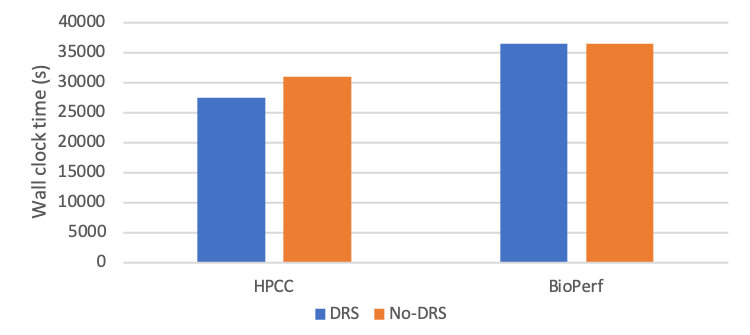
\includegraphics[width=\textwidth]{Figures/memory_wct}
         \caption{Wall clock time}
         \label{fig:memory_wct}
     \end{subfigure}
     \hfill
     \begin{subfigure}[b]{0.45\textwidth}
         \centering
         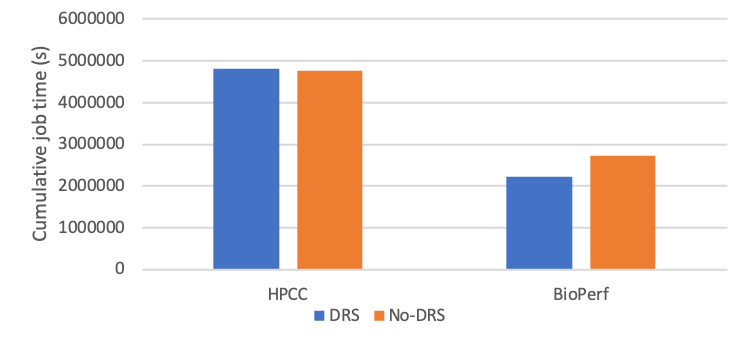
\includegraphics[width=\textwidth]{Figures/memory_cjet}
         \caption{Cumulative job execution time}
         \label{fig:memory_cjet}
     \end{subfigure}
     \caption{Comparison between DRS enabled and DRS disabled for VTC with 2X CPU and memory over-commitment. Workloads are from scenario 1. }
     \label{fig:memory_scenario1}
\end{figure}

As mentioned above, the second scenario is much more demanding because HPCC jobs can potentially consume all the configured VM memory. It's not a surprise the cluster is not able to finish two simultaneous streams of HPCC jobs, regardless of whether DRS is used. The guest OS encountered CPU soft lockup errors when hypervisor swapping occurs and when swapping is not responsive enough. Our analysis identified HPL (one benchmark in the HPCC suite) jobs as the bottleneck. Each HPL job needs more than 3 hours to finish, and once enough HPL instances accumulate on any node, the hypervisor is not able to handle their excessive memory requirements. Therefore, we decided to remove HPL from the job stream. After this change, we see that two HPCC streams can finish when DRS is on. Without DRS, the same failure occurs. Clearly, this demonstrates the effectiveness of DRS in load balancing and mitigating memory pressure. 

Though HPCC VMs are heavier to migrate, on average 67 VM migrations occurred per run, due to the extreme memory stress. Naturally, one may concern that the large number of migrations could introduce jitters to the running workloads. To quantify that, we collect the execution time distribution among all instances for each benchmark. It turns out that the execution time is quite consistent. For example, the histogram for RandomAccess (another benchmark in the HPCC suite) is shown in Figure~\ref{fig:ra_histogram}.

\begin{figure}[!t]
   \begin{center}
       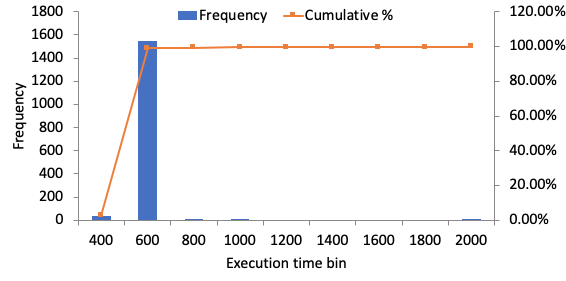
\includegraphics[width=\columnwidth]{Figures/ra_histogram}
   \end{center}
   \caption{Histogram of individual RandomAccess job execution time from both virtual clusters.}
   \label{fig:ra_histogram}
 \end{figure}






%\section{\uppercase{Tolerating crash and silent failures simultaneously}}
%\label{sec:multiple}
%It is well known that using $f+1$ replicas can tolerate $f$ crash failures and $2f+1$ can tolerate $f$ silent failures. Actually, it is not difficult to derive that $f_1 + 2f_2 + 1$ replicas can tolerate both crash and silent failures, assuming there are at most $f_1$ crash failure(s) and $f_2$ silent failure(s). We argue that the two schemes presented in Section~\ref{sec:crash_collocation} and~\ref{sec:silent_cp_leap} can be combined to tolerate both types of failures simultaneously, while reducing energy consumption under certain constraints. 


This section presents a case study that tolerates 1 crash failure and 1 silent failure, by using 4 replicas, which is the minimum number of replicas required. The execution dynamics are shown in Figure~\ref{fig:com_failure_model}. 
Two fast replicas will consume data from one end, and the two slow replica will proceed from the opposite end. Voting is invoked periodically to detect silent failure. If neither crash nor silent failure occurs, the four replicas will meet at a rendezvous point, determined by their relative execution rates (Figure~\ref{fig:com1}. 

\begin{figure}[!t]
	\begin{center}
		\subfigure[Non-faulty task.]
		{
			\label{fig:com1}
			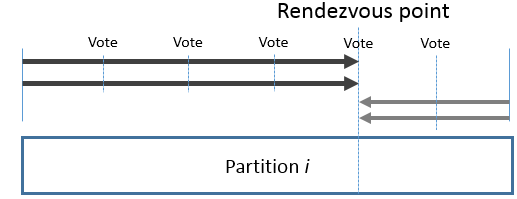
\includegraphics[width=0.9\columnwidth]{figures/combine1}
		}
		\subfigure[Task with a silent failure.]
		{
			\label{fig:com3}
			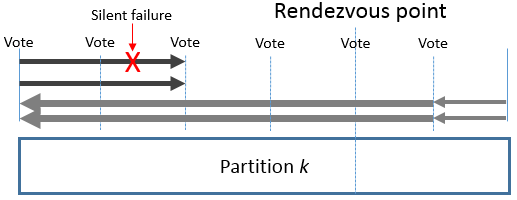
\includegraphics[width=0.9\columnwidth]{figures/combine3}
		}
        \subfigure[Task with a crash failure.]
		{
			\label{fig:com2}
			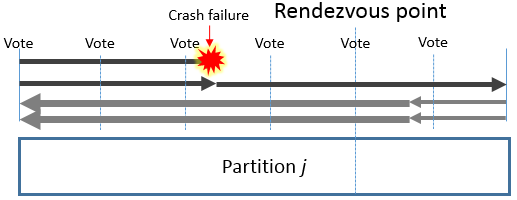
\includegraphics[width=0.9\columnwidth]{figures/combine2}
		}
	\end{center}
	\caption{Illustration of the tolerance of 1 crash failure and 1 silent failure simultaneously.}
	\label{fig:com_failure_model}
\end{figure}

If a failure occurs, there are two execution strategies, based on the type of the failure. If it is a silent failure, let's say a fast replica fails, then both fast replicas can be terminated when they reach an disagreement at the next voting point. In this case, however, the two slow replicas need to proceed beyond the original rendezvous point and process the whole partition, potentially at a higher rate to meet deadline, if any. With two remaining replicas, the system is still able to tolerate a crash failure. The illustration is shown in Figure~\ref{fig:com3}.

If the first failure occurred is a crash failure, a different execution strategy will be applied, as shown in Figure~\ref{fig:com2}. After a crash failure happens, all three remaining replicas need to continue execution and process the whole partition. This allows the system to detect and correct a subsequent silent failure. Similarly, the remaining replicas may speed up after the failure for response time consideration. 

\section{\uppercase{Related work}}
\label{sec:related_work}
%Extreme-scale computing presents some unique challenges to fault tolerance as faults are no longer 
%an exceptional event \cite{ferreira_sc_2011}. 
Rollback and recovery is the predominate mechanism to achieve fault
tolerance in current HPC environments. In the most general form, rollback and recovery 
involves the periodic saving of the current system state, with the anticipation that
in the case of a failure, computation can be restarted from the most recently saved state \cite{Elnozahy:02:Survey}. %The identification of an error, before or during a checkpoint,
%requires that the application rollback to the previously completed checkpoint. 
Coordinated checkpointing is a popular approach for
its ease of implementation.
%Specifically, all processes
%coordinate with one another to produce individual states that satisfy the ``happens before"
%communication relationship \cite{chandy_trans_1972}, which is proved to provide a consistent global state.
%Essentially, the algorithm provides a method for all processes involved to stop operation ``at the same
%time" and transfer their system state to a stable storage. 
%The major benefit of coordinated
%checkpointing stems from its simplicity and ease of implementation. 
Its major drawback, however, is the
lack of scalability, as it requires global coordination
\cite{elnozahy_dsc_2004,riesen_sandia_2010}.
%hargrove2006berkeley}.


In uncoordinated checkpointing, processes record their states independently and postpone creating a 
globally consistent view until the recovery phase. The major advantage is the reduced overhead during fault free operation. However, the scheme requires that
each process maintains multiple checkpoints and message logs, necessary to construct a consistent 
state during recovery. It can also suffer the well-known domino effect 
 \cite{randell_domino_effect}. One hybrid approach, known as communication induced 
checkpointing, aims at reducing coordination overhead \cite{alvisi_ftc_1999}. The approach, however, may 
cause processes to store useless states. To address this 
shortcoming, ``forced checkpoints" have been proposed \cite{helary_rds_1997}. This approach, however,  may lead to unpredictable
checkpointing rates. Although well-explored, uncoordinated checkpointing has not been widely adopted
in HPC environments, due to its dependency on applications \cite{guermouche_2011_ipdps}.


One of the largest overheads in any checkpointing process is the time necessary to write the checkpointing 
to stable storage. Incremental checkpointing attempts
to address this by only writing the changes since previous checkpoint \cite{Agarwal:04:Adaptive,elnozahy_1992_manetho,li_trans_1994}. %This
%can be achieved using dirty-bit page flags \cite{plank_ftcs_1994,elnozahy_1992_manetho}. Hash based incremental checkpointing, on the other
%hand, makes use of hashes to detect changes \cite{nam_ftc_1997,Agarwal:04:Adaptive}. 
Another proposed scheme, known as in-memory checkpointing, minimizes the overhead of disk access~\cite{zheng_2004_ftccharm}.
%offloads the checkpointing process to a secondary task and only writes incremental checkpoints \cite{li_trans_1994}.
The main concern of these techniques is the increase in
memory requirement to support the simultaneous execution of the checkpointing and the application. It has been suggested that nodes in extreme-scale systems should be configured with fast local storage~\cite{doe_ascr_exascale_2011}. 
%, which
%improves the performance of checkpointing \cite{doe_ascr_exascale_2011}. 
Multi-level checkpointing, which consists of
writing checkpoints to multiple storage targets, can benefit from such a strategy \cite{Moody:10:SCR}. This,
however, may lead to increased failure rates of individual nodes and complicate the checkpoint writing process.
%Furthermore, it may complicate the checkpoint writing process and requires that the system track the
%current location of all process's checkpoints.


Our work is based on process replication, or state machine replication, which has long been used to provide fault tolerance in distributed and mission critical systems\cite{schneider_1990_tutorial}. %Replication can be used to detect and correct system failures that are otherwise undetectable,
%such as silent data corruption and Byzantine faults \cite{fiala_2012_sdc}. 
Recently, replication has been proposed as a
viable alternative to checkpointing in HPC \cite{ferreira_sc_2011,Cappello:09:Fault,fiala_2012_sdc}. 
In addition, full and partial
replication have also been used to augment existing checkpointing techniques, and to guard
against silent data corruption \cite{stearly_2012_partial,elliott_2012_cpr}.% There are several different implementations of
%replication in the widely used MPI library, each with their different tradeoffs and overheads. The
%overhead can be negligible or up to 70\% depending upon the communication patterns of the
%application \cite{engelmann2011redundant}. %Moreover, replication alone is not enough to guarantee fault tolerance since
%it is possible that all nodes executing a given process could fail simultaneously, thus
%replication is typically paired with some form of checkpointing. 
The most relevant works to ours is redundant multi-threading (RMT) whereby one leading thread of execution is running ahead of trailing threads \cite{reinhardt2000transient,Wadden:2014:RDE:2665671.2665686}. However, our approach is different in that it tunes the execution rates of the leading and trailing threads in a finer grain, in order to achieve a ``parameterized" trade-off between completion time and energy consumption. Further, we take advantage of the idle time during failure recovery and ``leap" the trailing threads to achieve forward progress%, largely improving performance in terms of both completion time and energy consumption. 
. This differs from RMT, of which the ``leaping" of the trailing thread results in extra overhead.
%To the best of our knowledge,
%Lazy Shadowing is the first attempt to explore a state-machine replication based framework
%that achieves a fine-grained tradeoff between time and hardware redundancy while meeting resilience and
%power requirements.


\section{\uppercase{Conclusion}}
\label{sec:conclusion}
%Current fault-tolerance approaches rely exclusively on either time or hardware redundancy for recovery. Rollback recovery  exploits time redundancy but can incur significant delay and high energy cost. On the other hand, process replication relies on hardware redundancy and requires a significant increase in resources and  power consumption.

In this paper, we propose Rejuvenating Shadows as a novel power-aware fault tolerance model, which guarantees forward progress, maintains consistent level of resilience, and minimizes implementation complexity and runtime overhead. Empirical experiments demonstrated that the Rejuvenating Shadows model outperforms in-memory checkpointing/restart in both execution time and resource utilization, especially in failure-prone environments.

Leaping induced by failure has proven to be critical in reducing the divergence between a main and its shadow, 
%with respect to workload execution.
%Consequently, the time to recover from subsequent failures is reduced significantly. 
thus reducing the recovery time for subsequent failures. Consequently, the time to recover from a failure increases with failure intervals.  
Based on this observation, a proactive approach is to ``force" leaping when the divergence between a main and its shadow exceeds a specified threshold. 
In our future work, we will further study this approach to determine what behavior triggers forced leaping in order to optimize the average recovery time. 

%we will study forcing the shadDuring experimentation we noticed the problem that recovery time in Rejuvenating Shadows can become substantial when the failure interval is large (Figure~\ref{fig:single_failure}). To deal with this issue, we are studying the idea of ``forced leaping", which borrows the idea from periodic checkpointing and forces a leaping whenever failure has been absent for a long time, in order to reduce the divergence between mains and shadows. Optimal intervals for forced leaping will be explored to balance between runtime overhead and failure recovery overhead. 

%In the future we plan to explore the integration with fault prediction techniques and the viability of dynamic and partial shadowing for platforms where nodes exhibit different ``health" status, e.g., some nodes may be more reliable while others are more likely to fail~\cite{gainaru2012fault}. 
%With this taken into account, we can apply dynamic scheduling of shadows only for mains that are likely to fail, to further reduce the resource requirement. 
%Another future direction is to study complier-assisted program slicing for fault detection. Specifically, slices that are fraction of their mains can run lazily as shadows and provide fault detection capability with reasonable coverage. 





\section*{Acknowledgment}
This research is based in part upon work supported by the Department of Energy under contract DE-SC0014376. %Any opinions, findings, and conclusions or recommendations  expressed in this material are those of the authors and do not necessarily  reflect the views of the Department of Energy.


%This is added to reduce the spacing between ref items
\newcommand{\BIBdecl}{\setlength{\itemsep}{0.25 em}}
%%%%%%%%%%%%%%%%%

\bibliographystyle{IEEEtran}
\bibliography{IEEEabrv,main}  



% that's all folks
\end{document}


